% to choose your degree
% please un-comment just one of the following
\documentclass[bsc,frontabs,twoside,singlespacing,parskip,deptreport]{infthesis}     % for BSc, BEng etc.
% \documentclass[minf,frontabs,twoside,singlespacing,parskip,deptreport]{infthesis}  % for MInf

\usepackage{hyperref}
\usepackage{cite}
\usepackage{amsmath}
\usepackage{graphicx}
\usepackage{caption}
\usepackage{subcaption}
\usepackage{wrapfig}
\usepackage{tikz}
\usepackage{pgfplots}
\pgfplotsset{compat=1.12}

%\usetikzlibrary{arrows.meta,calc,decorations.markings,math,arrows.meta}

\pgfplotsset{percentgraph/.style={%
        width=0.93\textwidth,
        ylabel={\% Messages Delivered},
        ymin=0,ymax=100}}

\begin{document}

\title{Targeted Influence in Social Networks}

\author{Lewis Barker}

% to choose your course
% please un-comment just one of the following
%\course{Artificial Intelligence and Computer Science}
%\course{Artificial Intelligence and Software Engineering}
%\course{Artificial Intelligence and Mathematics}
%\course{Artificial Intelligence and Psychology }   
%\course{Artificial Intelligence with Psychology }   
%\course{Linguistics and Artificial Intelligence}    
\course{Computer Science}
%\course{Software Engineering}
%\course{Computer Science and Electronics}    
%\course{Electronics and Software Engineering}    
%\course{Computer Science and Management Science}    
%\course{Computer Science and Mathematics}
%\course{Computer Science and Physics}  
%\course{Computer Science and Statistics}    

% to choose your report type
% please un-comment just one of the following
%\project{Undergraduate Dissertation} % CS&E, E&SE, AI&L
%\project{Undergraduate Thesis} % AI%Psy
\project{4th Year Project Report}

\date{\today}

\abstract{
We consider the problem of trying to deliver messages to specific targets in a social network via re-sharing by other users. The problem is constrained by the limited attention span users, who can only process a small number of messages and share some of these each round. We design display algorithms which select messages to show to each user, with the goal of maximising the number of messages delivered. These algorithms are evaluated on various graph types, primarily Kleinberg's social network model. We find that algorithms which combine small deterministic choices with larger amounts of randomisation perform well. Additionally, the algorithms are run on a portion of a real social network. Performance on this network is found to be lower than using the model, however it is unclear whether this is caused by the social network being incomplete or differences between the model and real networks.
}

\maketitle

\tableofcontents

%\pagenumbering{arabic}


\chapter{Introduction}

This project considers the problem of delivering messages across a social network to specific targets via users' interactions. For example, consider the social network Facebook. Suppose User \textit{A} has a message they wish to show to User \textit{B}, but the two are not friends on Facebook. User \textit{A} could pay to have the message shown directly to \textit{B} as an advert, however it has been shown that people are more receptive of messages which are received from others who know rather than from corporate entities - such as in viral and word-of-mouth marketing \cite{viralmarketing, wordofmouth}. Therefore it would be better for \textit{A} if they were able to send the message somehow to another user who \textit{is} friends with \textit{B}, and have them show it to \textit{B}. To achieve this \textit{A} \textbf{shares} the message, allowing their friends to potentially see it. From here, some of their friends may also share the message, and it may propagate through the social network like this, eventually reaching \textit{B}.

\begin{figure}
\centering
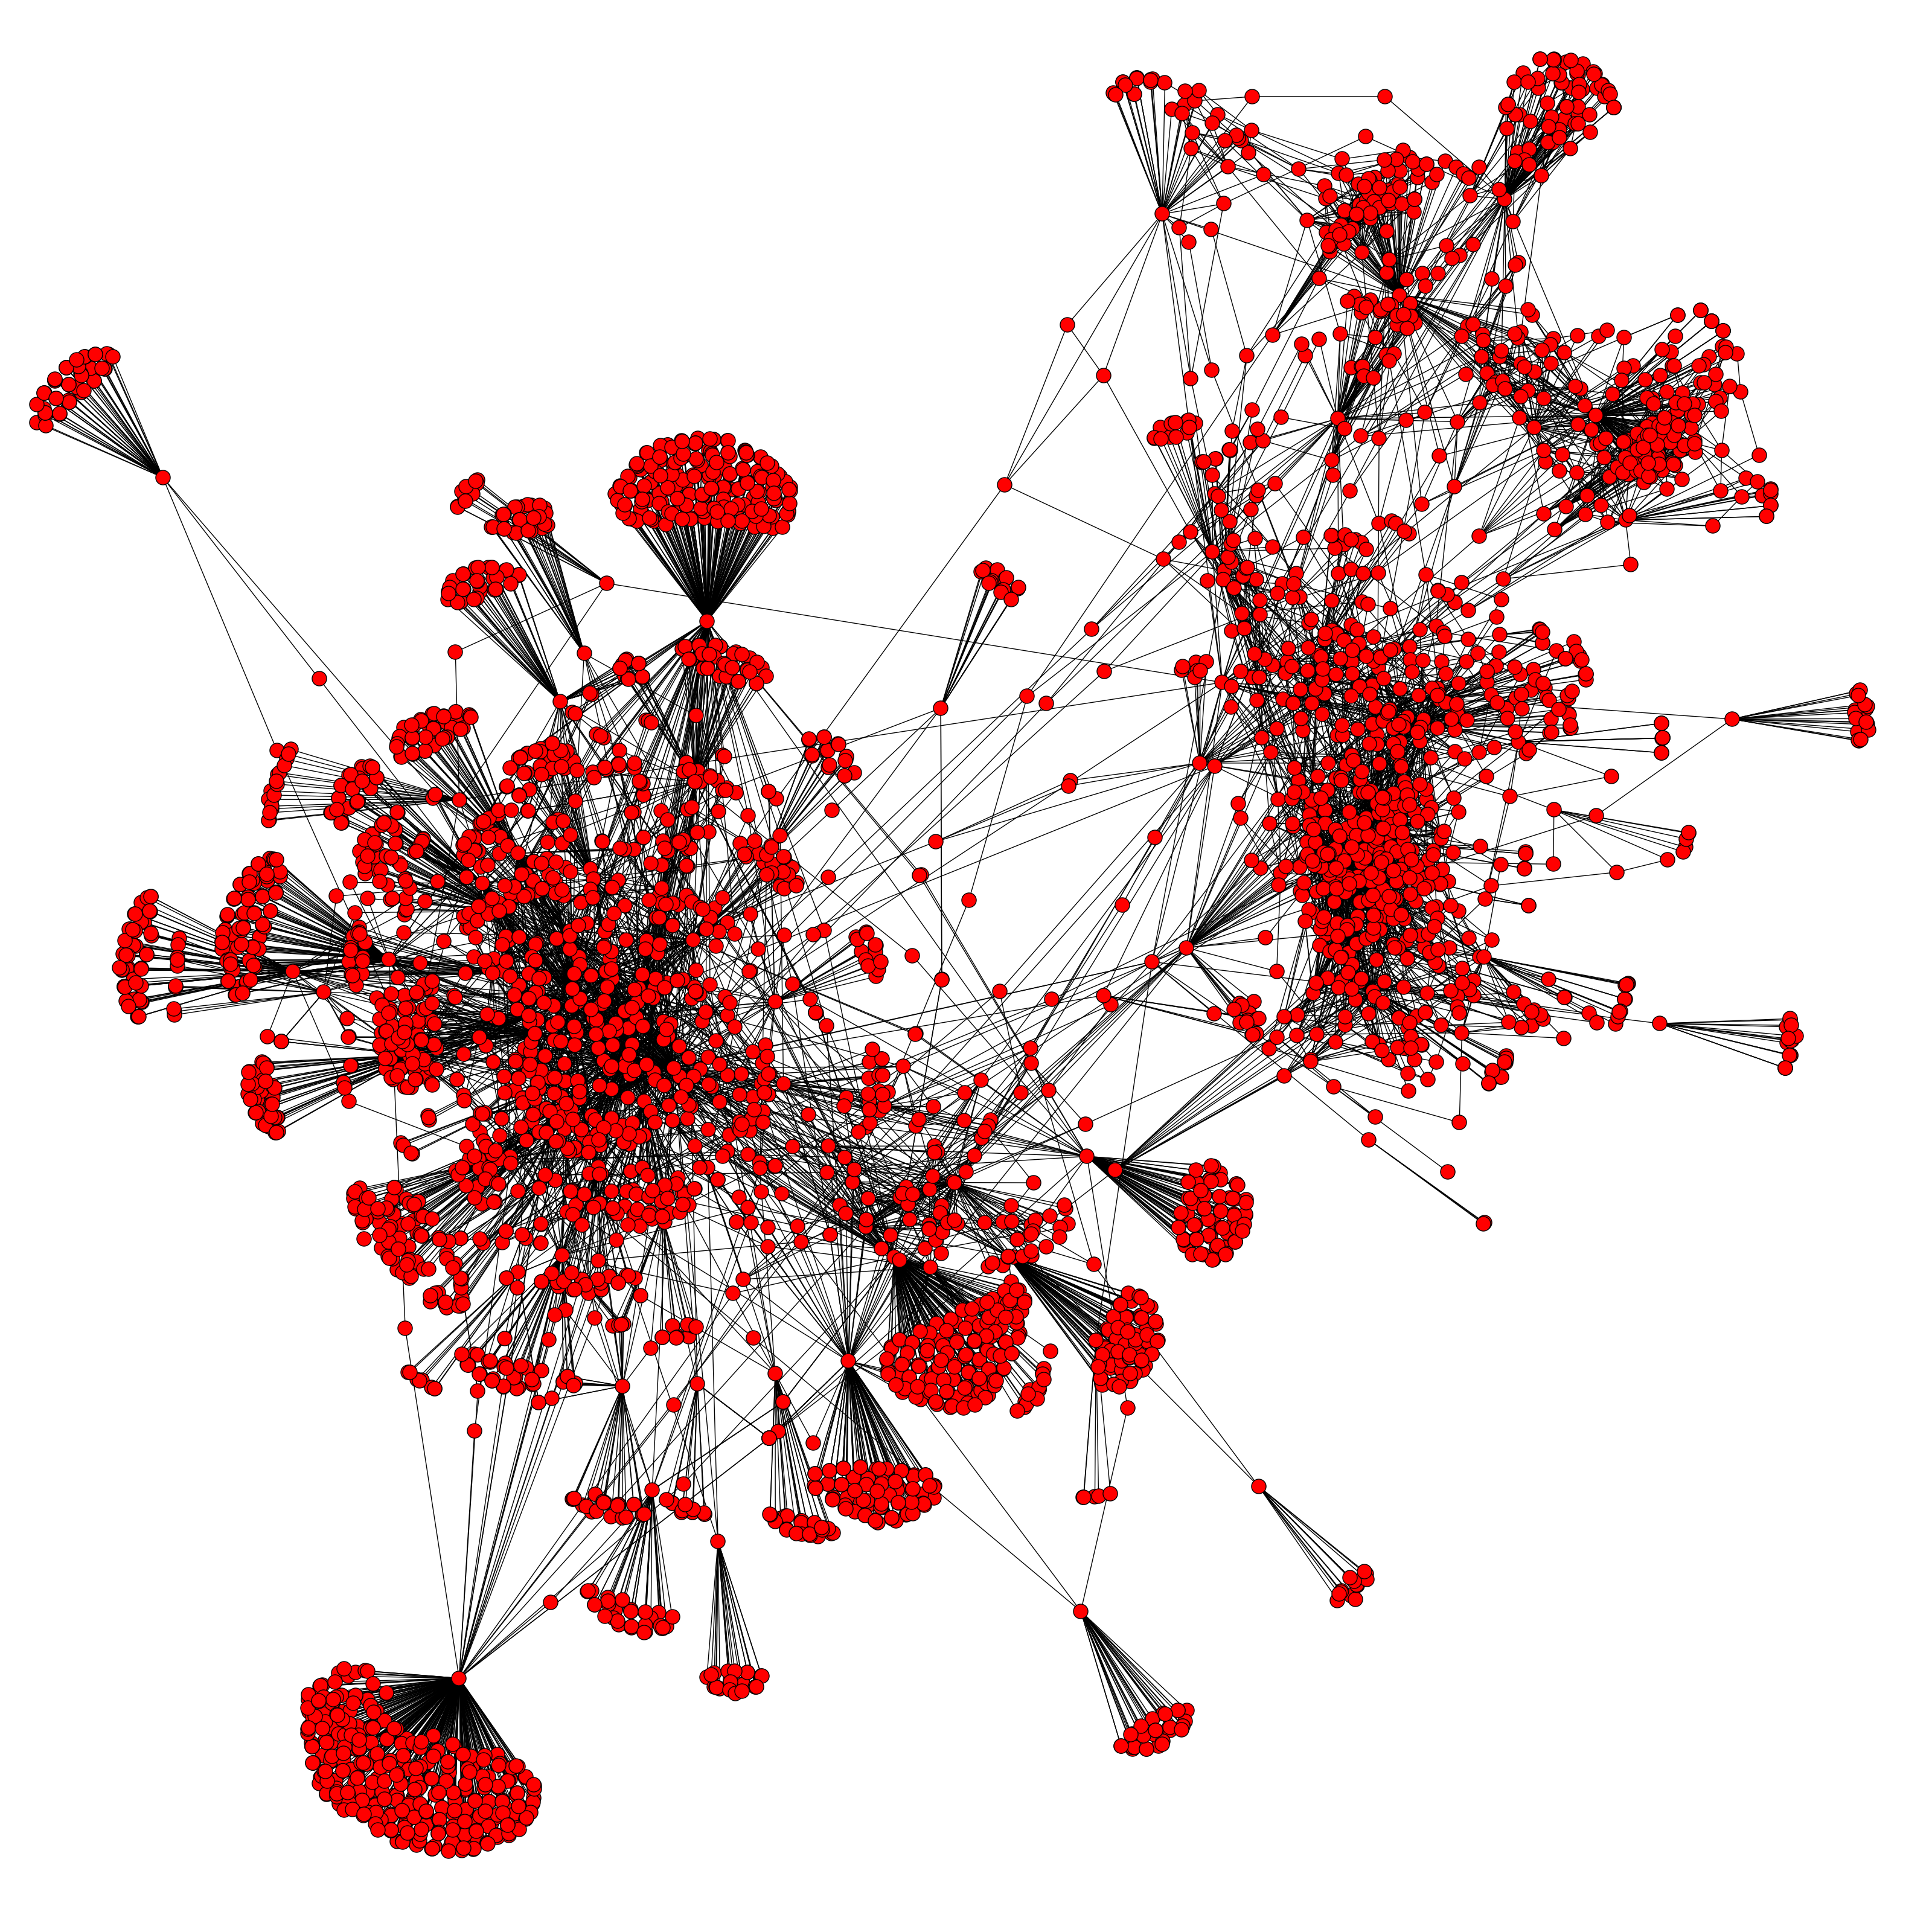
\includegraphics[width=0.45\textwidth]{pokec_4000}
\caption{Part of a real social network. This graph was extracted from the SNAP Pokec dataset\cite{snapnets}, and the developed display algorithms were tested on it.}
\label{fig:pokec_4000_intro}
\end{figure}

To improve the chances of the message reaching the destination, the social network's \textbf{display algorithm} can be utilised - this chooses which messages to show to each user from what their friends have shared. By considering destinations when making this choice, messages can be directed more efficiently, improving the number delivered.

An algorithm capable of delivering such messages has many applications. The most obvious use is for targeted advertising. While this type of information spread in social networks is often used for general viral marketing, it may be the case that making a specific user aware of some product is particularly advantageous. This method could be used to direct it to them, without it seeming like they are being shown ``adverts". This is particularly useful when considering users with large amounts of influence, such as a celebrity. Significant research has gone into identifying these influential users\cite{InfluenceMaximisation1, InfluenceMaximisation2, LabelledInfluenceMaximisation}. These studies generally consider how a message spreads from an initial user or set of users, and try to find those who maximise the spread of the message. In other words, if a message can be delivered to an influential user they can cause a cascade, allowing it to reach many others. This results of this project could be used to direct the message to those influential users.

A different approach could be to use this method in a more charitable way, such as raising awareness of a some cause. Again this can be done in a viral way using information spread in networks, and influential users could again be targeted to spread the message further. In addition however, certain individuals may be known to be at more risk of some condition, and so spreading awareness to them would be particularly effective. Alternatively, certain users in a social graph will be positioned in such a way that they have a high probability of detecting a ``contagion" spreading through it in early stages - identifying these users has been the subject of some research \cite{OutbreakDetection}. Spreading related information to these users may be an effective way to combat such contagions.

Finally, it may be possible to combine this method with graph summarisation techniques\cite{GraphSummary}. These involve condensing a large graph into a smaller one, in which super-nodes represent sets of nodes which had similar connections in the original graph. Using a summarised graph to represent the social network would still retain the connectedness properties that allow the method to work, but have other advantages. Communities would be targeted rather than individuals - for example rather than targeting a certain at-risk user with an awareness message, a group who are similarly at-risk might be targeted. This would also reduce the size of the problem, potentially making complex algorithms more feasible for large networks.

\begin{figure}
\centering
\begin{tikzpicture}
\begin{axis}[percentgraph,xmin=0,xmax=1,xlabel={fraction of messages chosen based on distance},width=0.55\textwidth,legend pos=outer north east]
\addlegendimage{empty legend}
\addplot table [x=Distance Priority Fraction, y=average delivered (percent), col sep=comma] {results/distance_priority_fraction/200messages.csv};
\addplot table [x=Distance Priority Fraction, y=average delivered (percent), col sep=comma] {results/distance_priority_fraction/400messages.csv};
\addplot table [x=Distance Priority Fraction, y=average delivered (percent), col sep=comma] {results/distance_priority_fraction/600messages.csv};
\addplot table [x=Distance Priority Fraction, y=average delivered (percent), col sep=comma] {results/distance_priority_fraction/800messages.csv};
\addplot table [x=Distance Priority Fraction, y=average delivered (percent), col sep=comma] {results/distance_priority_fraction/1000messages.csv};
\legend{\hspace{-.6cm}\textbf{Message Count},200,400,600,800,1000}
\end{axis}
\end{tikzpicture}
\caption{The fraction of messages shown to the user which are chosen based on which are closest to their destinations (with the remaining fraction picked randomly) is varied. The optimal value is found to be when 20\% of messages are picked based on distance and 80\% randomly. However even picking only one (5\%) based on distance gives almost as good results.}
\label{fig:distance_priority_fraction_intro}
\end{figure}

In this project we defined this system of message propagation via user interaction. We proposed several display algorithms, both deterministic and probabilistic, which were tested in simulations of the social network. We found that combining random and deterministic elements gives the best results, delivering more messages than either alone. Figure \ref{fig:distance_priority_fraction_intro} shows the results for such an algorithm, when varying the fraction of message shown to the user which are chosen deterministically. In this case a fraction are chosen based on which are closest to their destination (and most likely to be delivered successfully), and the remainder are picked at random. The best ratio was found to involve only a very small number of messages chosen based on distance, and even taking only a single distance-based message and all others at random performs close to the optimal found.

Additionally, we investigated the effect of different graph types on this process. Simple chains, trees and grids were considered, with the observation that the average degree of the nodes in the graph can play a more significant role in the ability of messages to spread and reach their targets than the delivery algorithm used can. If the nodes do not have enough connection, then it becomes very hard for the message to properly spread. Lastly, the algorithms developed were tested on a graph created from a part of a real social network, shown in figure \ref{fig:pokec_4000_intro}. We found that algorithms which performed well on Kleinberg's social network model did not perform as well on the portion of the real social network used. However it was unclear whether this was due to flaws in the method of extracting a part of the social network or if it was caused by differences between the model and real social networks.


\section{Challenges}
Even though we are able to choose what to show to each user to help deliver messages, there are several potential problems. When using social networks, users will not see everything that their friends share - they will likely only look at some of the top items on their ``news feed" before running out of attention. If there are a large number of messages shared by a user's friends then since not all of them will be seen, not all of them can be passed on. To ensure that as many messages reach their target as possible, the amount of ``noise" seen by a user must be reduced - in other words we only show a message  where it is beneficial to delivering that message, to avoid clogging up the network. This is achievable by utilising the fact that in most social networks a user's ``news feed", rather than being random, is generated by some complex algorithm. By modifying this algorithm and deciding what to show to each user, messages can be directed towards their destinations.

Since each message only needs to reach the destination once, the best way to reduce noise might be to find the shortest path from source to destination, and show it only to the next user along this path at each step. The problem with this is that even among those messages seen by a user, they may not share them all for one reason or another. Over enough steps a single copy of a message will likely get lost, and so it must be duplicated to increase the chance of delivery as much as possible. The algorithm now has to balance duplication of messages to avoid loss and avoiding unnecessary noise due to duplication.

\begin{figure}
\begin{subfigure}[]{0.48\textwidth}
\centering
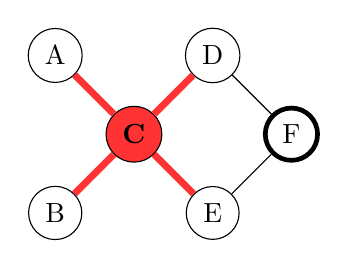
\begin{tikzpicture}
    \node[shape=circle,draw=black] (A) at (0,2) {A};
    \node[shape=circle,draw=black] (B) at (0,0) {B};
    \node[shape=circle,draw=black,fill=red!80!white] (C) at (1,1) {\textbf{C}};
    \node[shape=circle,draw=black] (D) at (2,2) {D};
    \node[shape=circle,draw=black] (E) at (2,0) {E};
    \node[shape=circle,draw=black, line width=1.7] (F) at (3,1) {F};
    
    %\path[color=blue, line width = 2.5] (A) edge (B);
    \path[line width=2.5, color=red!80!white] (A) edge (C);
    \path[line width=2.5, color=red!80!white] (B) edge (C);
    \path[line width=2.5, color=red!80!white] (C) edge (D);
    \path[line width=2.5, color=red!80!white] (C) edge (E);
    \path (D) edge (F);
    \path (E) edge (F);
\end{tikzpicture}
\caption{Initially user $C$ has a message with the destination user $F$. They share the message, potentially allowing any of their neighbours to see it.}
\end{subfigure}
\quad
%
\begin{subfigure}[]{0.48\textwidth}
\centering
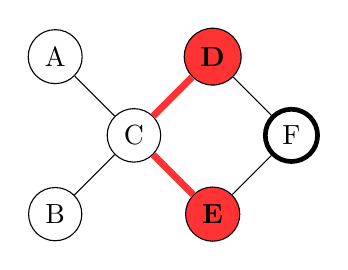
\begin{tikzpicture}
    \node[shape=circle,draw=black] (A) at (0,2) {A};
    \node[shape=circle,draw=black] (B) at (0,0) {B};
    \node[shape=circle,draw=black] (C) at (1,1) {C};
    \node[shape=circle,draw=black,fill=red!80!white] (D) at (2,2) {\textbf{D}};
    \node[shape=circle,draw=black,fill=red!80!white] (E) at (2,0) {\textbf{E}};
    \node[shape=circle,draw=black, line width=1.7] (F) at (3,1) {F};
    
    %\path[color=blue, line width = 2.5] (A) edge (B);
    \path (A) edge (C);
    \path (B) edge (C);
    \path[line width=2.5, color=red!80!white] (C) edge (D);
    \path[line width=2.5, color=red!80!white] (C) edge (E);
    \path (D) edge (F);
    \path (E) edge (F);
\end{tikzpicture}
\caption{We show $D$ and $E$ the message that was shared by $C$. Users $A$ and $B$ are further from the destination, so we do not bother showing the message to them.}
\end{subfigure}
%
\par\bigskip 
%
\begin{subfigure}[]{0.48\textwidth}
\centering
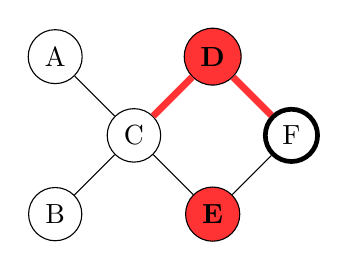
\begin{tikzpicture}
    \node[shape=circle,draw=black] (A) at (0,2) {A};
    \node[shape=circle,draw=black] (B) at (0,0) {B};
    \node[shape=circle,draw=black] (C) at (1,1) {C};
    \node[shape=circle,draw=black,fill=red!80!white] (D) at (2,2) {\textbf{D}};
    \node[shape=circle,draw=black,fill=red!80!white] (E) at (2,0) {\textbf{E}};
    \node[shape=circle,draw=black, line width=1.7] (F) at (3,1) {F};
    
    %\path[color=blue, line width = 2.5] (A) edge (B);
    \path (A) edge (C);
    \path (B) edge (C);
    \path[line width=2.5, color=red!80!white] (C) edge (D);
    \path (C) edge (E);
    \path[line width=2.5, color=red!80!white] (D) edge (F);
    \path (E) edge (F);
\end{tikzpicture}
\caption{User $D$ shares the message, but $E$ does not. This is outside of our control, and can't be predicted.}
\end{subfigure}
\quad
%
\begin{subfigure}[]{0.48\textwidth}
\centering
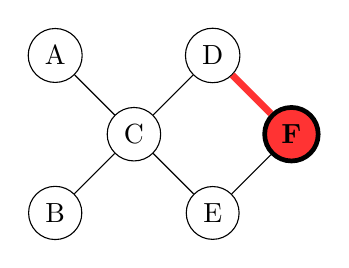
\begin{tikzpicture}
    \node[shape=circle,draw=black] (A) at (0,2) {A};
    \node[shape=circle,draw=black] (B) at (0,0) {B};
    \node[shape=circle,draw=black] (C) at (1,1) {C};
    \node[shape=circle,draw=black] (D) at (2,2) {D};
    \node[shape=circle,draw=black] (E) at (2,0) {E};
    \node[shape=circle,draw=black, line width=1.7,fill=red!80!white] (F) at (3,1) {\textbf{F}};
    
    %\path[color=blue, line width = 2.5] (A) edge (B);
    \path (A) edge (C);
    \path (B) edge (C);
    \path (C) edge (D);
    \path (C) edge (E);
    \path[line width=2.5, color=red!80!white] (D) edge (F);
    \path (E) edge (F);
\end{tikzpicture}
\caption{We can now show the message that $D$ shared to $F$, the destination user. The message is now successfully delivered.}
\end{subfigure}
\caption{An example of how a message can travel across the network to reach its destination.}
\label{fig:intro_example}
\end{figure}

This problem can be formalised using a graph to represent the social network, and having a number of messages at each node at any time in the process. The messages then move from one node to the next based on algorithms used to describe the actions of the user and the social network. Figure \ref{fig:intro_example} shows an example of this with a single message. Here red nodes have the message, blue nodes do not, and the yellow node is the target. The message moves through adjacent nodes until it reaches the target. We wish to choose which nodes to show the messages to at each step so as to maximise the overall number of messages delivered.


\section{Related Literature}
At the core of this project is spreading information within a network. This is and similar concepts have been investigated in many forms. For example, ``rumour spreading" involves attempting to spread messages to \textit{every} node in a network. An early example of this is \cite{Pittel87}, which looks at spreading a single rumour to all of a population of involved people. The paper uses a process consisting of discrete rounds, in which each individual who is informed of the rumour passes it on to another participant at random (who may or may not already be informed). The number of rounds required for there to be a high probability that the rumour spreads from a single person to all people involved are investigated, and a bound on this is proved. In \cite{KarpSSV00} a similar process is investigated, again looking at spreading a single rumour to all participants. A random phone call model is used, in which every round each player contacts another at random. In the \textit{push} scheme the caller passes the rumour on to the callee (as in \cite{Pittel87}), and in the \textit{pull} scheme rumours are only spread from callee to caller. A \textit{push\&pull} scheme combines these, allowing information to spread in either direction. A further more advanced scheme is also considered, which spreads the rumour in a more robust manner. Both of these papers looks at similar concepts to this project, however they differ in several ways. Both allow any player to contact any other, rather than having a social network of allowed communication; and both focus on spreading a single message to every player rather than many messages to specific targets.

There are also studies on spreading information in this way through social networks. An example is \cite{SocialNetworkRumours}, which considers the push and pull schemes as described above, but does so within a Preferential Attachment network, used to simulate a social network. This makes it more similar to the graph-based problem this project investigates, however again it only considers single messages spreading to all users.

An aspect of this project which is less common in literature is considering the limited attention of users in the network. A form of this is investigated in \cite{AllocatingAttention}. Rather than using rounds, content is created and users consult their neighbours (using a pull scheme) according to Poisson processes. The attention limit is in the form of a limit to the sum of a user's rates of consulting their neighbours - however within this limit, attention may be allocated as desired. Cost for each user is defined in terms of how quickly any new content reaches them, and a social cost for the whole network in terms of how quickly content reaches all users. The paper investigates the cost when each user allocates their attention selfishly (to minimise their own cost) compared to the optimal cost, for several different graph types. This is similar to the system considered in this project - multiple messages interact at once, and users cannot see all of them at once due to limited attention. However the continuous process and lack of targets make the way the system is considered quite different.

Another less common aspect is targeting users within the social network. In \cite{TargetedSignedNetworks} this idea of sending a message from source to target is investigated, but in the context of signed networks. Here each connection in the social graph is either ``positive" or ``negative" - signifying the type of relationship between the two individuals. If a message is passed to a user via someone they have a negative relationship with, then it will cause the recipient to lean towards the opposite view - and then that opposite view may be passed across another negative relationship, returning to the original. The paper looks at algorithms to create a path from the source to destination which minimises the distance while resulting in a positive influence on the target. While this contains the targeting aspect of this project's problem, the users in this paper are assumed to act in the optimal way which the algorithm wants them to - there is no random interactions. In this sense, while the algorithm may still be useful in some cases, it is a less realistic approach.

\section{Overview}
In Chapter \ref{chapter2} we present a formal definition of the problem model used. We then describe the graph types used, and define the user models, display algorithms, and distance measures.

Chapter \ref{chapter3} we describe the implementation of the model simulation which is used to run our experiments.

Chapter \ref{chapter4} covers the various experiments we carried out and their results. Section \ref{sec:user_model_comparison} compares the two user models described, and we discuss why the probabilistic model is more appropriate. In Section \ref{sec:display_alg_comparisons} we present experiments comparing the various display algorithms, and in Section \ref{sec:distance_measure_comparisons} we build on this by also considering different distance measures that can combined with display algorithms. In Section \ref{sec:other_graph_types} we investigate how these algorithms perform on simpler graphs - chains, trees, and grids - and what this suggest about them and the model used. In section \ref{sec:real_social_network} we describe how a subgraph was extracted from a real social network, and the results of running our algorithms on this network.

Finally Chapter \ref{chapter5} concludes this report and suggests some possibilities for future work on this subject.


\chapter{Formal Definitions} \label{chapter2}

Before any algorithms can be developed, we need to define the problem formally. This describes the process by which messages are spread through the graph, and how the user model and display algorithms (the algorithms which decides on messages to show each user) affect this.

With the problem itself clearly defined, we then look at the other aspects of the system which can change:
\begin{itemize}
\item The \textbf{network graphs} used to run simulations on. The algorithms described can be used with any kind of graph, however for most experiments Kleinberg's model is used. This is due to being a known standard, which generates random graphs matching certain properties of social networks.
\item The \textbf{user models}, which decide the messages that are shared by users out of those shown to them.
\item The \textbf{display algorithms}, which decide the messages to show to each user out of those shared by their friends. These algorithms are designed with the intention of delivering as many messages as possible.
\item The \textbf{distance measures}, which are used as part of the display algorithms to define how ``close" nodes are to each other.
\end{itemize}

All of these aspects are formally defined within this section.

\section{Problem Model}

\begin{figure}
\centering
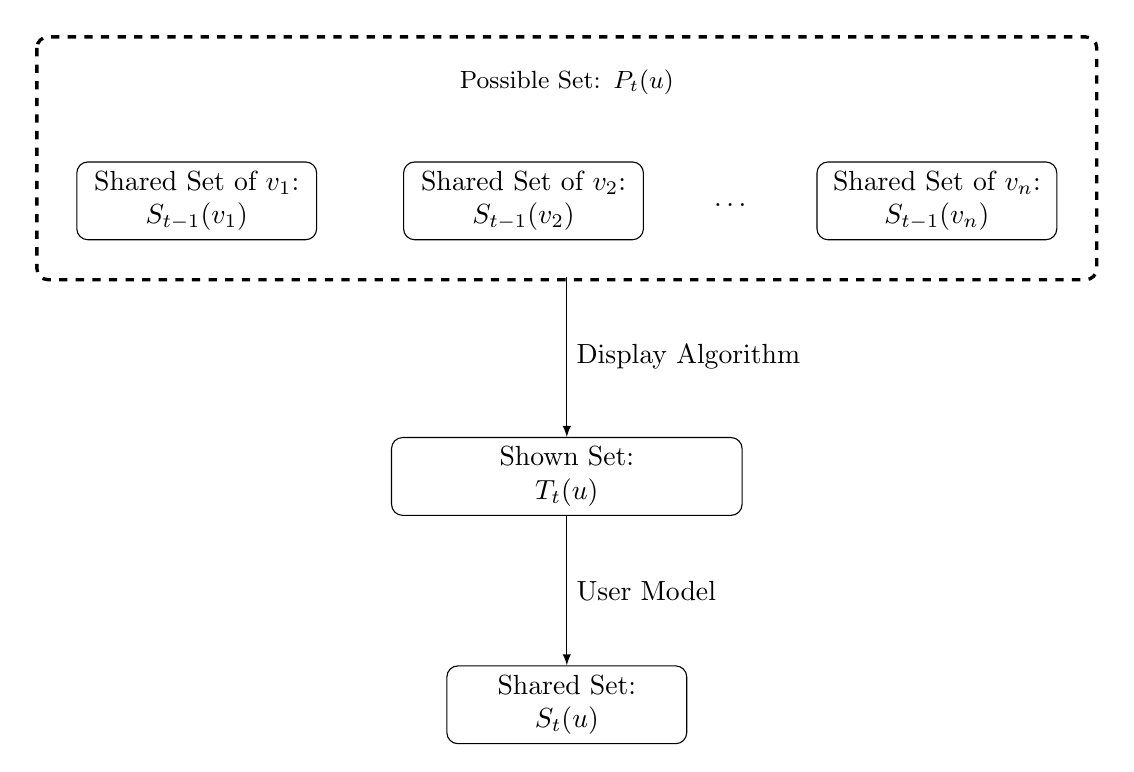
\begin{tikzpicture}
\pgfdeclarelayer{background}
\pgfsetlayers{background,main}

\node (shown) [draw, text centered, minimum height=1em, text width=12em, rounded corners]  {Shown Set:\\ $T_{t}(u)$};

\node[text width=4cm, text centered,font=\small] at (0,5) (possible) {Possible Set: $P_{t}(u)$};

\path (-4.7,3.5) node (neighbour1) [draw, text width=8em, text centered, minimum height=2.5em, rounded corners] {Shared Set of $v_1$:\\ $S_{t-1}(v_{1})$};
\path (-0.55,3.5) node (neighbour2)[draw, text width=8em, text centered, minimum height=2.5em, rounded corners] {Shared Set of $v_2$:\\ $S_{t-1}(v_{2})$};
\path (2.075,3.3) node (dots)[above, text width=6em, text centered] {$\hdots$}; 
\path (4.7,3.5) node (neighbour3)[draw, text width=8em, text centered, minimum height=2.5em, rounded corners] {Shared Set of $v_n$:\\ $S_{t-1}(v_{n})$}; 

\path (0,-2.9) node (shared)[draw, text width=8em, text centered, minimum height=1em, rounded corners] {Shared Set:\\ $S_{t}(u)$}; 

\draw[-{latex}] (shown.south) -- node[right] {User Model} (shared.north);

\begin{pgfonlayer}{background}
    \path (neighbour1.west |- possible.north)+(-0.5,0.3) node (a) {};
    \path (neighbour3.east |- neighbour3.south)+(+0.5,-0.5) node (b) {};
          
    \path[rounded corners, draw=black, dashed, line width=1.2] (a) rectangle (b) node (rect) {};
\end{pgfonlayer}

\path (shown.north |- rect)+(+0,+0.16) node (c) {};
\draw[-{latex}] (c) -- node[right] {Display Algorithm} (shown.north);

\end{tikzpicture}
\caption{The process of message spreading, where $v_{1}$ to $v_{n}$ are the neighbours of $u$. The \textbf{shown set} of $u$ is formed from a subset of their neighbours' shared sets from the previous round, using the \textbf{display algorithm}. The \textbf{shared set} of $u$ is then formed from a subset of their shown set, using the \textbf{user model}}
\label{fig:algorithms_flowchart}
\end{figure}

Initially we are given a \textbf{graph} $G = (V, E \subseteq V \times V)$ and $k$ \textbf{messages} $ m_{1} ... m_{k}$, which have \textbf{sources} $s_{1} ... s_{k}$ and \textbf{destinations} $d_{1} ... d_{k}$. In our model, these messages are assigned sources and destinations randomly at the beginning of the process.

The graph $G$ represents the social network, with vertices in $V$ being the users of the network and edges in $E$ being connections between users within the network. A connection between two users $u$ and $v$ means in our context that user $u$ may potentially see some content shared by user $v$ - however other factors may stop this. Out aim is to direct messages through the network so that as high a percentage as possible are seen by their final target.

The system progresses in a series of \textbf{rounds}, representing periods of time passing in which messages can be passed on to other users. This allows us to more easily reason about the flow of information and also simulate the process.

For any round $t$, and for some vertex $v \in V$, the \textbf{shared set} $S_{t}(v)$ is the set of messages which were shared by $v$ in that round. We assume that the source of a message will invariably share it initially (otherwise it has no chance to propagate). Therefore initially, at round 0, for each $v \in V$ the shared set is defined as the set of messages for which $v$ is the source:

\begin{equation}
S_{0}(v) = \{m_{x} \:\: | \:\: x \in [0, k] \:\: and \:\: s_{x} = v\}
\end{equation}


Let $N(v)$ be the set of neighbouring vertices of v, and $(u, m)$ is a 2-tuple. Given a tuple $p = (u, m)$, we say that $p_{(1)} = u$ and $p_{(2)} = m$, as a way of accessing the parts of the tuple. Using this we define, for each $v \in V$ at any round $t > 0$, the \textbf{possible set} as all of the messages shared by neighbours of $v$ in the previous round - all the messages which $v$ could potentially be shown at this point:

\begin{equation}
P_{t}(v) = \bigcup_{u \in N(v)} \:\:\:\: \bigcup_{m \in S_{t-1}(u)} (u, m)
\end{equation}

Which of these messages are actually shown to $v$ is determined by the social network's \textbf{display algorithm} - which is what we wish to design. We define the \textbf{shown set} of a user $v$ at some round $t$, $T_{t}(v)$, as the result of this algorithm - this will be a subset of the possible set for that user and round:

\begin{equation}
T_{t}(v) \subseteq P_{t}(v)
\end{equation}

Finally, from the messages that are shown to a user, the user will share some of them. This is decided by the user model algorithm. The result of this form the \textbf{shared set} of that user for this round - all messages in the user's shared set must have been part of their shown set for that round:

\begin{equation}
\forall m \in S_{t}(v) .\; \exists (u, n) \in T_{t}(v) .\; m = n
\end{equation}

This is then used as the basis for the possible set of neighbouring vertices in the next round. With this, we need only define the display algorithm and user model to be able to simulate the spread of messages throughout the network. Note that if in some a particular message is not shared by any user (whether this is due to it not being shown to anyone or the user model algorithm not selecting any instance of it) then that message will not be present in any possible sets for the next round. As a result it cannot be shown to any more users, and if it was not already delivered can never be delivered. A diagram of this process is shown in Figure \ref{fig:algorithms_flowchart}.

\section{Network Graphs} \label{sec:graph_def}
An important factor in how a display algorithm performs is the network that it is being performed on. If the network has invalid properties, a successful algorithm may not be successful on other networks.

\subsection{Kleinberg's Model}

For the majority of this project, Kleinberg's model for small world graphs is used\cite{Kleinberg00}. This is a model which randomly creates a graph that fits certain properties. Initially, nodes are arranged in a grid layout. The grid or Manhattan distance between two nodes is defined as the shortest number of steps that must be taken along the original grid to get from one node to another. Each node is connected to its immediate neighbours (those a grid distance of 1 away). Each node is then connected to a constant number $k$ of other nodes. The probability of connecting node $u$ to node $v$ in this way is proportional to $d(u, v)^{-q}$ where $d(u, v)$ is the grid distance between $u$ and $v$, and $q$ is a constant affecting how likely the links are to be ``far-reaching". If $q$ is 0, then the node will be linked to other nodes uniformly. If $q$ is high, the long links are more likely to connect closer nodes.

\begin{figure}[]
  \centering
    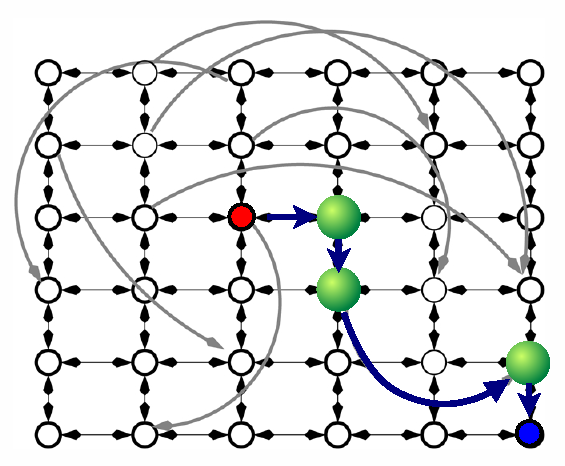
\includegraphics[width=0.5\textwidth]{Schabanel11_Kleinbergs_Network}
  \caption{A Kleinberg graph with an example of the distributed greedy search - Figure re-used from \cite{Schabanel11}}
\end{figure}

This model provides several properties which make it suitable to use in place of a social network. Since it is randomly generated, we can run experiments using multiple different graphs to avoid results being skewed by peculiarities of individual networks. Additionally it fits into a category of graphs know as ``Small World" graphs. This is related to Milgram's famous ``Six Degrees of Separation" experiment\cite{Milgram67,TraversMilgram69}, in which he randomly chose individuals and asked them to forward a message on to a certain ``target" via people they knew. Of those messages that reached the target, the median number of ``steps" required was 6, displaying the existence of short paths within social networks - a fact that has also been seen in other studies\cite{MilgramBackup1,MilgramBackup2}. In addition to these paths existing, the experiment showed that it was possible for the intermediate individuals to find these paths without knowing the full structure of the network - they were able to conduct a distributed search. 

Kleinberg's model replicates both of these properties. For $q = 2$ and $k \ge 1$ the expected diameter of a graph generated using this model is $\theta (\log n)$ and a route between two nodes can be found in a distributed manner using $\theta (\log^{2}n)$ steps\cite{AnalyzingKleinberg}. This is achieved by sending the message as close as possible to the destination (in terms of grid distance) at each step.

This can be related to real networks intuitively. Individuals are more likely to be connected to those ``close" to them - which in turn forms clusters of connections - but there will also be some ``long-distance" connections that can connect clusters. To send a message to a far away target, a reasonable strategy would be to send to the person you know who is ``closest" to the target - they are more likely to be connected to them.

\subsection{Other Graph Types}

While we primarily use Kleinberg's small world model, other graph types are also considered for the sake of learning more about how messages spread in simpler situations. We consider three other graph types:

\begin{itemize}
\item \textbf{Chain Graphs}: A simple chain of nodes each connected to the next and previous. This provides information about the simplest case, where there are minimal connections available.
\item \textbf{Tree Graphs}: Specifically, we use complete, balanced, binary trees. This provides a similar case to chains in terms of simplicity and minimal number of connections, but has shorter paths between nodes with less overlap.
\item \textbf{Grid Graphs}: Since Kleinberg's graph model is a grid with some added connections, we also consider a plain grid to see what effect these extra links have.
\end{itemize}

\section{User Models} \label{sec:user_models}
While the main focus of this project is on the effect of the social network's display algorithm, the model used also requires an algorithm to represent the user's actions. This algorithm should decide which of the messages shown to a user they then share - it chooses $S_{t}(v)$ based on $T_{t}(v)$. Depending on how this decision is modelled, it can add an element of uncertainty or randomness to the system, affecting which display algorithms perform well.

\subsection{Basic User Model}
Initially, a very basic random selection method was used to choose $S_{t}(v)$. Firstly, the user only actually sees and considers the top $a$ of the messages shown to them (or all of the messages if there is less than $a$), where $a$ is a global constant - this represents the user's ``attention", being unable to look at every message shown to them. To In the implementation used, the value of $a$ is also known to the display algorithm, which does not show more than this many messages. From these $a$ messages, $b$ are selected at random and shared (or all of them are shared if there are less than $b$), where $b$ is a global constant and $b \le a$. More formally:

\begin{equation}
S_{t}(v) = sample(T_{t}(v)[:a], \; min(|T_{t}(v)|,\: b))
\end{equation}

Where $x[:a]$ is the first $a$ items in $x$ and $sample(x, n)$ randomly samples $n$ values from the collection $x$.

This provides us with a degree of randomness - if there are more than $b$ messages shown to the user, we can't tell which ones will be passed on. However in the case where there are less than or equal to $b$ messages shown to the user, this model acts unrealistically - the user will share every message they see. A real social network user would likely be less predictable (unless there was some incentive to share messages), and may not share all of the messages in nay circumstances. As a result of this unnatural behaviour, showing each message to only a single user at each step was found to be a highly effective strategy - however in a real situation this would likely result in losing the message at an uncooperative user.

\subsection{Probabilistic User Model}
A more realistic user model can be created using probabilistic methods. In this user model, the concept of a maximum attention of $a$ is retained, with the user considering up to $a$ messages. However from these $a$ messages, rather than choose a set amount at random each message is shared with a probability $p_{share}$, where $p_{share}$ is a global constant. This simulates the way that users will choose whether or not to share each message based on what they like, or some other similar criteria. Since the reasoning behind these choices are unknown to us, they are effectively random. More formally:

\begin{equation}
S_{t}(v) = \{x \in T_{t}(v)[:a] \:\: | \:\:  r < p_{share}\}
\end{equation}

Where the previous definition of $x[:a]$ applies, and $0 \leq r < 1$ is a value chosen at random each time it is inspected. 

This results in a situation where a user may share all the messages they see, or may share none. This emulates more closely how an actual user will only share certain messages based on some criteria unknown to the network - these unknown criteria are modelled over all users in general by this probabilistic sharing. With this model, if messages are not spread to a sufficiently large number of users then they are likely to not be shared at some point and be lost. We therefore consider this model to be more suitable for use in simulations than the basic one.

\section{Display Algorithms} \label{sec:display_algorithms}
The key part of this project is the algorithm which decides which messages to show to each user. Users have ``attention" limits, meaning that they will only look at a certain (globally constant) number of messages each round. This means that we can't just pass on every message - we need to prioritise. Each user is therefore only shown messages up to the ``attention limit" to represent this. By changing which messages are shown we can attempt to direct messages to their recipients, preferably without clogging up the network with numerous duplicates and without losing the message by not duplicating it enough.

Several algorithms have been investigated, using relatively basic heuristics to decide whether or not to show a message to a user. In all of these algorithms, when considering possible message to show to a user, those which have already been delivered are discounted. To simplify this, we define $Q_{t}(v)$ as the set of sender-message pairs from $P_{t}(v)$ where the message has not been delivered. In the non-formal descriptions, delivered messages are implicitly discounted unless otherwise stated.

Almost all of these algorithms use some sense of ``distance" between nodes. There are several ways to define this distance, each giving different performance - for detail on these see Section \ref{sec:distance_measures}. For the sake of defining the display algorithms this ``distance measure" is left general, and we use $D(u, v)$ to represent the distance between two nodes in whatever measure is used. In simulations a distance measure must be chosen to be used as part of the display algorithm.

Note that in some of these algorithm, if a message is in the possible set multiple times (from different previous nodes), it may be shown to the user multiple times (once for each previous node). Depending on the user model, this may increase the probability of it being shared by them.

\subsection{Algorithm 1: Any Closer Node}

\begin{wrapfigure}{r}{0.4\textwidth}
\centering
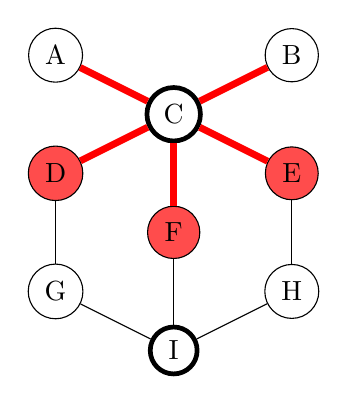
\begin{tikzpicture}
    \node[shape=circle,draw=black] (A) at (0,3.75) {A};
    \node[shape=circle,draw=black] (B) at (3,3.75) {B};
    \node[shape=circle,draw=black, line width=1.7] (C) at (1.5,3) {C};
    \node[shape=circle,draw=black,fill=red!70!white] (D) at (0,2.25) {D};
    \node[shape=circle,draw=black,fill=red!70!white] (E) at (3,2.25) {E};
    \node[shape=circle,draw=black,fill=red!70!white] (F) at (1.5,1.5) {F};
    \node[shape=circle,draw=black] (G) at (0,0.75) {G};
    \node[shape=circle,draw=black] (H) at (3,0.75) {H};
    \node[shape=circle,draw=black, line width=1.7] (I) at (1.5,0) {I};
    
    \path[color=red, line width = 2.5] (A) edge (C);
    \path[color=red, line width = 2.5] (B) edge (C);
    \path[color=red, line width = 2.5] (C) edge (D);
    \path[color=red, line width = 2.5] (C) edge (E);
    \path[color=red, line width = 2.5] (C) edge (F);
    
    \path (D) edge (G);
    \path (F) edge (I);
    \path (E) edge (H);
    
    \path (G) edge (I);
    \path (H) edge (I);

    
\end{tikzpicture}
\caption{In this example, $C$ has a message bound for $I$. They share the message (shown by red edges), which using Algorithm 1 (Any Closer Node) is made a candidate to be shown to $D$, $E$, and $F$, who are all closer to the destination.}
\label{fig:alg_1_example}
\end{wrapfigure}

In the first algorithm used, for each node we first select candidate messages that may be shown to them. A message is made a candidate if the receiving node (the one potentially being shown the message) is closer to the message's final target than the previous node is (the one that shared this message in the previous round, causing it to be part of the possible set). In other words, the messages progress only to nodes which are closer to the destination. After candidates have been selected, if there are more messages than can be shown to the node, the maximum amount are chosen randomly from the candidates. 

More formally, we first define $a$ as the maximum number of messages that can be shown to any one node (their attention span) and $sample(x, n)$ as a random sample of $n$ values from the set $x$. The shown set can be then be defined as follows:

\begin{equation}
\begin{split}
candidates_{t}(v) = \{ (u, m_{k}) \in Q_{t}(v) \:\: | \:\: & D(v, d_{k}) < D(u, d_{k}) \}
\end{split}
\end{equation}

\begin{equation}
T_{t}(v) = sample(candidates_{t}(v), min(|candidates_{t}(v)|, a))
\end{equation}

An example of this algorithm is shown in Figure \ref{fig:alg_1_example}.

\subsection{Algorithm 2: Further Nodes With Probability}
\usetikzlibrary{patterns}

\begin{wrapfigure}{l}{0.4\textwidth}
\centering
\begin{tikzpicture}
	\node[shape=circle,draw=black,preaction={fill, white},pattern=north west lines,pattern color=red!70!white] (A) at (0,3.75) {A};
    \node[shape=circle,draw=black,preaction={fill, white},pattern=north west lines,pattern color=red!70!white] (B) at (3,3.75) {B};
    \node[shape=circle,draw=black, line width=1.7] (C) at (1.5,3) {C};
    \node[shape=circle,draw=black,fill=red!70!white] (D) at (0,2.25) {D};
    \node[shape=circle,draw=black,fill=red!70!white] (E) at (3,2.25) {E};
    \node[shape=circle,draw=black,fill=red!70!white] (F) at (1.5,1.5) {F};
    \node[shape=circle,draw=black] (G) at (0,0.75) {G};
    \node[shape=circle,draw=black] (H) at (3,0.75) {H};
    \node[shape=circle,draw=black, line width=1.7] (I) at (1.5,0) {I};
    
    \path[color=red, line width = 2.5] (A) edge (C);
    \path[color=red, line width = 2.5] (B) edge (C);
    \path[color=red, line width = 2.5] (C) edge (D);
    \path[color=red, line width = 2.5] (C) edge (E);
    \path[color=red, line width = 2.5] (C) edge (F);
    
    \path (D) edge (G);
    \path (F) edge (I);
    \path (E) edge (H);
    
    \path (G) edge (I);
    \path (H) edge (I);

    
\end{tikzpicture}
\caption{Again, $C$ shares a message bound for $I$. Using Algorithm 2 (Further Nodes With Probability) it is made a candidate to be shown to $D$, $E$, and $F$; but also made a candidate for $A$ and $B$ with probability $p_{further}$ each - shown by partially shaded nodes.}
\label{fig:alg_2_example}
\end{wrapfigure}

The second algorithm is a modification of the first with the intention of allowing the messages to spread in other directions not necessarily towards their destination. This may help prevent the message from dying out if the ``direct" route is very busy, by creating additional duplicates.

In this algorithm, we again select candidates to be shown to each node. Any message for which the receiving node is closer to the destination than the previous node is made a candidate, as before. Additionally, messages which will not get closer to their destination are made candidates with a globally constant probability. As before, if there are too many candidates then the correct amount are chosen at random.

We define $0 \leq p_{further} < 1$ as a globally constant probability and $0 \leq r < 1$ as a value chosen at random each time it is inspected. This allows us to describe the algorithm as follows:

\begin{equation}
\begin{split}
candidates_{t}(v) = \{ (u, m_{k}) \in Q_{t}(v) \:\: | \:\: & (D(v, d_{k}) < D(u, d_{k}) \quad or \quad r < p_{further}) \}
\end{split}
\end{equation}

\begin{equation}
T_{t}(v) = sample(candidates_{t}(v), \; min(|candidates_{t}(v)|, \: a))
\end{equation}

Note that if $p_{further}$ were to be set to 0, Algorithm 2 would behave the exact same as Algorithm 1. An example of this algorithm is shown in Figure \ref{fig:alg_2_example}.

\subsection{Algorithm 3: Only Best Node}

The third algorithm uses a simpler concept - each message is passed on to at most one other node, which is always the node that is determined to be the ``best" next step. This is used mainly for comparing other algorithms to this case, where messages are never duplicated.

Candidate messages are again selected for each node. In this algorithm we make a message a candidate to be shown to a node only if that node is the ``best" next step for the message. We define the ``best" next step as the neighbour of the previous step (the only node which has this message) that is closest to the target, and in the case of a draw has the lowest node index (to ensure that the ``best" next step is consistent). If there are more than $a$ candidates then the first up to $a$ are taken. Since we are not worried about spreading messages ``fairly" as they do not duplicate, this doesn't need to be chosen randomly. 

We define $isBest(m, u)$ as a predicate which is true if node $u$ is the best next step for message $m$, and $x[:a]$ as the first $a$ items in $x$. The shown set is then calculated as follows:

\begin{equation}
\begin{split}
candidates_{t}(v) = \{ (u, m_{k}) \in Q_{t}(v) \:\: | \:\: & isBest(m_{k}, u) \}
\end{split}
\end{equation}

\begin{equation}
T_{t}(v) = candidates_{t}(v)[:a]
\end{equation}

An example of this algorithm is shown in Figure \ref{fig:alg_3_example}.

\begin{figure}[h]
\centering
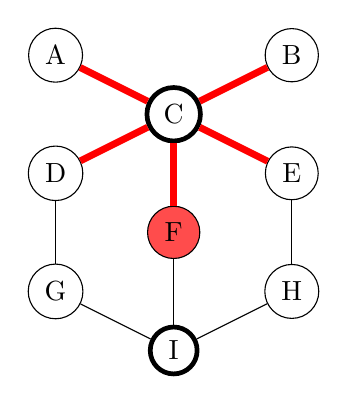
\begin{tikzpicture}
	\node[shape=circle,draw=black] (A) at (0,3.75) {A};
    \node[shape=circle,draw=black] (B) at (3,3.75) {B};
    \node[shape=circle,draw=black, line width=1.7] (C) at (1.5,3) {C};
    \node[shape=circle,draw=black] (D) at (0,2.25) {D};
    \node[shape=circle,draw=black] (E) at (3,2.25) {E};
    \node[shape=circle,draw=black,fill=red!70!white] (F) at (1.5,1.5) {F};
    \node[shape=circle,draw=black] (G) at (0,0.75) {G};
    \node[shape=circle,draw=black] (H) at (3,0.75) {H};
    \node[shape=circle,draw=black, line width=1.7] (I) at (1.5,0) {I};
    
    \path[color=red, line width = 2.5] (A) edge (C);
    \path[color=red, line width = 2.5] (B) edge (C);
    \path[color=red, line width = 2.5] (C) edge (D);
    \path[color=red, line width = 2.5] (C) edge (E);
    \path[color=red, line width = 2.5] (C) edge (F);
    
    \path (D) edge (G);
    \path (F) edge (I);
    \path (E) edge (H);
    
    \path (G) edge (I);
    \path (H) edge (I);

    
\end{tikzpicture}
\caption{Once again, $C$ shares a with destination $I$. Using Algorithm 3 (Only Best Node), it is only made a candidate for $F$, which is the closest choice.}
\label{fig:alg_3_example}
\end{figure}

\subsection{Algorithm 4: Distance Priority}
The previous algorithms looked at how far a message is from its destination, but only in terms of whether or not a single step takes it closer - there is not consideration of how much closer it gets. They also treat all messages equally regardless of how close to their destination they currently are - however a message that is only two steps from the destination is far more likely to get delivered than one which is ten steps away. To maximise the overall number of messages delivered, it may be advantageous to greedily prioritise those which are closer to their destination.

This algorithm achieves both prioritising long links (in a sense) and prioritising nearly-delivered messages. It does this using a simple method - we order the messages that can be shown to a user $v$, $P_{t}(v)$, by the distance from $v$ to the destination of that message. The closest $a$ items are then shown to the user, where $a$ is the user's attention limit (or if there are less than $a$ possible messages, all are shown). Long links are not specifically prioritised, however travelling a (useful) long link should take a message significantly closer to its destination, and so is generally more likely to be chosen at any point in time than a short link starting from the same place.

To describe this formally, we define a ranking $R_{dist}(u, m)$, the ranking of messages in $Q_{t}(v)$ by the distance from $u$ to the destination of $m$. For any two messages $m_{i}, m{j} \in Q_{t}(v)$, if $D(u, d_{i}) < D(u, d_{j})$ then $R_{dist}(u, m_{i}) > R_{dist}(u, m_{j})$. The closest message to its destination is given the rank 0, and ranks increase from there. In the case of a draw (where two messages would be the same distance from their destination) then they are ordered arbitrarily in the ranking (but still have distinct ranks). The algorithm can then be described as follows:

\begin{equation}
T_{t}(v) = \{ (u, m_{k}) \in Q_{t}(v) \:\: | \:\: R_{dist}(v, m_{k}) < a \}
\end{equation}

In other words, up to $a$ of the lowest ranking (closest) messages are shown to the user.

\subsection{Algorithm 5: Fractional Distance Priority}
While algorithm 4 prioritises messages which are close to their destination, this is done at the expense of others - if the network has many messages, those which are almost delivered will be propagated many times and use up the the attention limit of users and prevent message which are further away from spreading. If a message that is far from its destination can reach a long link then it will quickly be delivered, but it must survive up to that point. This algorithm uses the prioritisation method of algorithm 4 for quick focused delivery, but also setting aside some capacity for keeping messages alive.

We achieve this by defining a fraction $f$ of each user's attention limit $a$ to be used for ``focused" delivery. From each node's possible set of messages, $a \times f$ are chosen based on which are closest to their destination. Of the remaining unpicked messages, $a - (a \times f)$ (the amount of attention still unused) are chosen at random. The first $a \times f$ messages accomplish the fast delivery of messages close to their destination, while the other $a - (a \times f)$ are used to keep other messages alive.

Formally, we first define $a_{priority} = a \times f$ as the number of messages which will be chosen based on the distance - this is rounded down if not a whole number. We also define $a_{random} = a - a_{priority}$, the number of messages chosen randomly.

We then split the set of possible message into two parts, those which are to be the portion chosen by distance and the remaining possible messages:

\begin{equation}
priority_{t}(v) = \{ (u, m_{k}) \in Q_{t}(v) \:\: | \:\: R_{dist}(v, m_{k}) < a_{priority} \}
\end{equation}
\begin{equation}
others_{t}(v) = \{ (u, m_{k}) \in Q_{t}(v) \:\: | \:\: R_{dist}(v, m_{k}) >= a_{priority} \}
\end{equation}

We choose the random selection of messages:

\begin{equation}
random_{t}(v) = sample(others_{t}(v), \; min(|others_{t}(v)|, \: a_{random}))
\end{equation}

Finally, we combine these two to produce our shown set:

\begin{equation}
T_{t}(v) = priority_{t}(v) \; \cup \; random_{t}(v)
\end{equation}

Note that if $f$ were to be set to 1, Algorithm 5 would behave the exact same as Algorithm 4.


\section{Distance Measures} \label{sec:distance_measures}
Many of the display algorithms described in Section \ref{sec:display_algorithms} involve some measure of distance $D(u, v)$ between two nodes $u$ and $v$. There a various ways to define this distance, depending on the desired properties and the graph type in use. Multiple different distance measures were used for experiments, to investigate how they affect the performance of the display algorithm.

\subsection{Grid Distance}
The most simplistic distance measure was based on the work done by Kleinberg in \cite{Kleinberg00}, the paper in which the Kleinberg graph model was proposed. In this paper a routing scheme for decentralised message delivery (with individual messages forwarded one node at a time) is outlined. The method used is simply to use the local knowledge of position within the graph - in the real world this may be geographical location, but in the graph it is represented using the position of the node in the original grid. Messages are forwarded to the neighbour who is closest to the destination in terms of lattice (or Manhatten) distance in this grid. If the $x$ and $y$ positions of a node $u$ in the grid are represented by $u_{x}$ and $u_{y}$, then this can be defined as follows:

\begin{equation}
D(u, v) = abs(u_{x} - v_{x}) + abs(u_{y} - v_{y})
\end{equation}

Where $abs(x)$ is the absolute value of $x$.

For graph types which are based on a grid, such as the Kleinberg model, this Manhatten grid distance can be used to determine the ``distance" between two nodes. This has the advantage of being very quick to compute, and also is possible using only local information at each node (although in this case we have centralised information anyway). However it is rather simplistic, and does not take into account the structure of the other parts of the graph, such as long links in the Kleinberg model.


\subsection{Graph Distance} \label{subsec:graph_dist}

\begin{wrapfigure}{r}{0.4\textwidth}
\centering
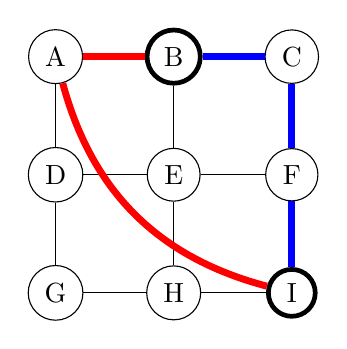
\begin{tikzpicture}
    \node[shape=circle,draw=black] (A) at (0,3) {A};
    \node[shape=circle,draw=black, line width=1.7] (B) at (1.5,3) {B};
    \node[shape=circle,draw=black] (C) at (3,3) {C};
    \node[shape=circle,draw=black] (D) at (0,1.5) {D};
    \node[shape=circle,draw=black] (E) at (1.5,1.5) {E};
    \node[shape=circle,draw=black] (F) at (3,1.5) {F};
    \node[shape=circle,draw=black] (G) at (0,0) {G};
    \node[shape=circle,draw=black] (H) at (1.5,0) {H};
    \node[shape=circle,draw=black, line width=1.7] (I) at (3,0) {I};
    
    \path[color=red, line width = 2.5] (A) edge (B);
    \path[color=blue, line width = 2.5] (B) edge (C);
    \path (D) edge (E);
    \path (E) edge (F);
    \path (G) edge (H);
    \path (H) edge (I);

    \path (A) edge (D);
    \path (D) edge (G);
    \path (B) edge (E);
    \path (E) edge (H);
    \path[color=blue, line width = 2.5] (C) edge (F);
    \path[color=blue, line width = 2.5] (F) edge (I);
    
    \path[color=red, line width = 2.5] (A) edge [bend right] (I);
\end{tikzpicture}
\caption{A case where using graph distance can find a shorter route than grid distance. If $B$ is the source and $I$ the target, the graph distance path has length 2 (shown in red), while a grid distance path has length 3 (shown in blue).}
\label{fig:graph_dist_example}
\end{wrapfigure}

With the use of centralised knowledge, a more accurate measure of distance than the simplistic grid measure can be created. This is done by using the length of the shortest path between any two nodes as their distance - equivalent to the minimum number of rounds for a message to travel between the nodes. By directing messages based on this measure it is possible to find shorter paths that don't necessarily follow the ``direction" towards the target within the grid - taking some steps in another direction may allow the use of convenient non-grid edges. This method also has the advantage of being usable for any kind of graph, whereas the grid distance measure required the graph to be based on a grid.

Figure \ref{fig:graph_dist_example} shows an example of a simple graph where graph distance is able to find a shorter path that grid distance. In the case where a message is at $B$ with the destination $I$, although the node $A$ is further from the destination in terms of grid distance, it leads to a useful long link which results in a shorter route overall.

\subsection{Diffusion Distance} \label{subsec:diffusion_dist}

A possible downside of the graph distance is that in some cases it relies on the specific shortest route being taken. Although following shorter paths to the destination can be found, they may involve taking long links to a point that is far away from the destination in the grid, with only a single other long link leading back towards it. Since users may fail to share messages, there is no guarantee that a single step in the route will be successful - and if multiple specific steps in a row are required to be successful, the probability of any failing becomes high. Therefore ideally, a message's ``next step" should not only be closer to the destination, but also have multiple routes leading to it - allowing for the message to be duplicated and some instances to be lost.

This problem is avoided in the grid distance measure, as any step taken closer to the destination will always still have short links leading towards it. These will be closer to reaching it than the short links at a the previous node, and there will almost always be a large number of possible paths that do not rely on specific edges.

\begin{wrapfigure}{R}{0.43\textwidth}
\centering
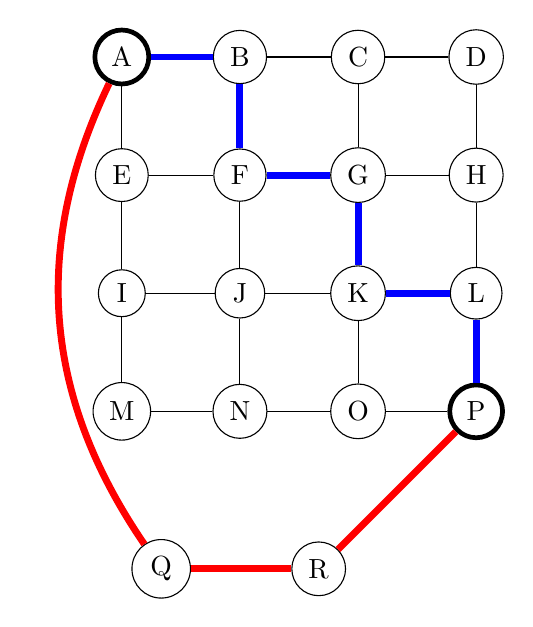
\begin{tikzpicture}
    \node[shape=circle,draw=black, line width=1.7] (A) at (0,4.5) {A};
    \node[shape=circle,draw=black] (B) at (1.5,4.5) {B};
    \node[shape=circle,draw=black] (C) at (3,4.5) {C};
    \node[shape=circle,draw=black] (D) at (4.5,4.5) {D};
    \node[shape=circle,draw=black] (E) at (0,3) {E};
    \node[shape=circle,draw=black] (F) at (1.5,3) {F};
    \node[shape=circle,draw=black] (G) at (3,3) {G};
    \node[shape=circle,draw=black] (H) at (4.5,3) {H};
    \node[shape=circle,draw=black] (I) at (0,1.5) {I};
    \node[shape=circle,draw=black] (J) at (1.5,1.5) {J};
    \node[shape=circle,draw=black] (K) at (3,1.5) {K};
    \node[shape=circle,draw=black] (L) at (4.5,1.5) {L};
    \node[shape=circle,draw=black] (M) at (0,0) {M};
    \node[shape=circle,draw=black] (N) at (1.5,0) {N};
    \node[shape=circle,draw=black] (O) at (3,0) {O};
    \node[shape=circle,draw=black, line width=1.7] (P) at (4.5,0) {P};
    \node[shape=circle,draw=black] (Q) at (0.5,-2) {Q};
    \node[shape=circle,draw=black] (R) at (2.5,-2) {R};
    
    \path[color=blue, line width = 2.5] (A) edge (B);
    \path (B) edge (C);
    \path (C) edge (D);
    \path (E) edge (F);
    \path[color=blue, line width = 2.5] (F) edge (G);
    \path (G) edge (H);
    \path (I) edge (J);
    \path (J) edge (K);
    \path[color=blue, line width = 2.5] (K) edge (L);
    \path (M) edge (N);
    \path (N) edge (O);
    \path (O) edge (P);

    \path (A) edge (E);
    \path (E) edge (I);
    \path (I) edge (M);
    \path[color=blue, line width = 2.5] (B) edge (F);
    \path (F) edge (J);
    \path (J) edge (N);
    \path (C) edge (G);
    \path[color=blue, line width = 2.5] (G) edge (K);
    \path (K) edge (O);
    \path (D) edge (H);
    \path (H) edge (L);
    \path[color=blue, line width = 2.5] (L) edge (P);
    
    \path[color=red, line width = 2.5, bend right] (A) edge (Q);
    \path[color=red, line width = 2.5] (Q) edge (R);
    \path[color=red, line width = 2.5] (R) edge (P);
\end{tikzpicture}

\caption{An example where using the graph distance may give poorer delivery rates. In the case where a message is at $A$ with the destination $I$, rather than the shortest route (shown in red), taking the longer routes through the grid (a possibility shown in blue) may reduce the chance of the message being lost by allowing duplication.}
\label{fig:diffusion_dist_example}
\end{wrapfigure}

An example is shown in Figure \ref{fig:diffusion_dist_example}. If a message is currently at $A$, and the destination is $P$, then the shortest path using graph distance is via $Q$ and $R$. However this requires both $Q$ and $R$ to share the message after it is shown to them, which (depending on the probability of sharing) may leave a significant probability of failure. On the other hand, if a slightly longer path through the grid-like part of the graph is taken, the message can easily be duplicated amongst the various other nodes in between. However measuring by graph distance puts both $B$ and $E$ further from the destination than $A$ is, so in several of the display algorithms used this route would be unlikely to be taken. A similar situation can arise in Kleinberg's graph model, where nodes taking the role of $Q$ and $R$ are very far away from the destination in the grid, and so delivering via them requires the use of specific long links.

To deal with this problem of some short paths requiring the exact route be taken without failure, diffusion distance can be used as an alternative distance measure. This method uses random walks to determine the distance between two nodes - if the random walks starting at either node have a good chance to end up in the same places, then the nodes are deemed ``close". This means that nodes with multiple paths between them are more likely to be ``close" to each other in this measure, as the chance of a random walk taking one of several paths is better than that of it taking a single specific path.

More specifically, to find the diffusion distance between $u$ and $v$ we first find the probability for random walks of some specific length $t$ starting at each to end in at any node in the graph. A problem with this can arise in cases where the probabilities of a random walk ending at any node do not reach an equilibrium. For example if a bipartate graph (such as a grid) is used, then for any value of $t$ the random walk can only end at nodes on one ``side" of the graph (depending on whether $t$ is odd or even). Two nodes from opposite ``sides" would therefore never have their random walks meet, and be deemed infinitely far apart. To combat this, ``lazy" random walks are used, where there is a 0.5 probability at each step of the walk staying in the same place.

Given this, the transition matrix for the lazy random walk (the probability of moving from one node to another) is given by:

\begin{equation}
\textbf{Z} = 0.5 \times (\textbf{I} + \textbf{D}^{-1} \times \textbf{A})
\end{equation}

Where $\textbf{A}$ is the graph's adjacency matrix, $\textbf{D}$ is the graph's diagonal degree matrix, and $\textbf{I}$ is the identity matrix (containing only 1s along the diagonal) of the same size as $\textbf{A}$ and $\textbf{D}$. In this matrix, $\textbf{Z}[i, j]$ is the probability of a random walk at node $i$ moving to node $j$ in the next step, where the graph nodes are indexed in some way. We then take $\textbf{Z}^{t}[i, j]$ to get the probability of a random walk starting at $i$ ending at $j$ after $t$ steps.

\pagebreak

To compare two nodes we take the row vectors containing the probabilities for random walks starting at each of these nodes, and find the difference between these vectors:

\begin{equation}
D(u, v) = \sum_{w=1}^{|V|} (\textbf{Z}^{t}[u, w] - \textbf{Z}^{t}[v, w])^{2}
\end{equation}

Where $|V|$ is the number of nodes in the graph.

\chapter{Implementation} \label{chapter3}
For the purpose of evaluating the developed algorithms, a program was written which allowed various simulations to be run, giving the desired results. The program was written in Python, using the NetworkX library\cite{NetworkX} to represent and manipulate network graphs. The program is split into classes, many of which have abstract base classes, to allow for easily creating and substituting different versions.

For most cases the network graph used was randomly generated from certain parameters, which remained constant. To allow for easy generation of these graphs each time a simulation was run, the \texttt{GraphGenerator} abstract base class was used. Subclasses encapsulate the knowledge specific to the graph model being used - including how to create instances, and how nodes should be positioned if visualised (for example if the network is based on a grid layout, it should be positioned as such). The rest of the program is totally independent from this knowledge, meaning using a different subclass allows a completely different graph generation process. Some instances that were used include creating Kleinberg graphs based on the parameters, creating copies of non-random graphs, and loading specific graphs from files.

User models are represented by subclasses of the \texttt{ShareModel} class, which has a method \texttt{share\_alg} to takes the user's shown set and return the messages which the user will share. Similarly, the display algorithms themselves are contained within subclasses of the \texttt{ShowModel} class, the \texttt{show\_alg} method of which, given a user's possible set and some additional information about the state of the network, can be called to decide the subset of messages to be shown to them. Since any display algorithm can be combined with any distance measure, this too is separated out to a different class. Subclasses of \texttt{DistanceMeasure} can implement different version of the \texttt{distance} method, which will return the distance between to nodes in a graph using that measure. Display algorithms then take a DistanceMeasure object as a parameter when they are created.

These classes are brought together by the \texttt{Simulation} class, which is given an instance of each of \texttt{GraphGenerator}, \texttt{ShowModel}, and \texttt{ShareModel} on creation. The simulation can then be either run once or repeated multiple times, with the results returned to the program and, if desired, written to a file. It is also possible to run multiple different simulations with a parameter varying and output the results to a file and a graph. In some cases it was desirable to have a full record of the simulation process. To achieve this, additional data can be saved to disk, which includes details on the simulation parameters and a record of which messages were shown to and shared by each node at every round.

\begin{figure}
\centering
\begin{subfigure}[]{0.47\textwidth}
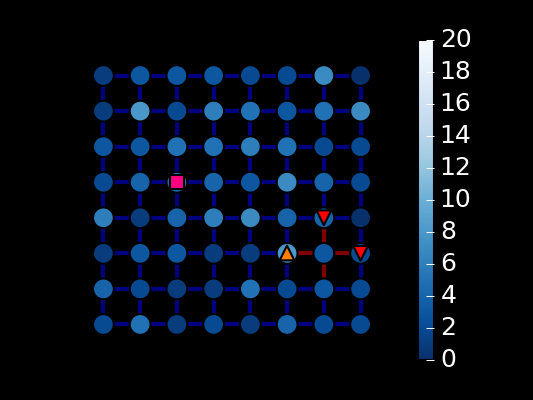
\includegraphics[width=0.99\textwidth]{visualisation_1}
\caption{The two nodes which are closer to the destination, and one which is further away, are shown the message. Of the 3 nodes who see the message, only one shares it.}
\end{subfigure}
\quad
\begin{subfigure}[]{0.47\textwidth}
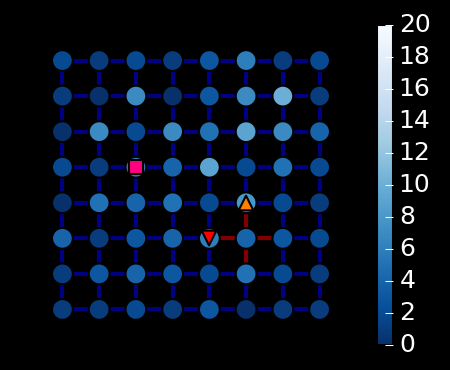
\includegraphics[width=0.99\textwidth]{visualisation_2}
\caption{The red edges now represent the connections from the node which shared the message last round. Two more nodes are shown the message, one of which shares it.}
\end{subfigure}
\caption{Part of a visualisation of the probabilistic user model and Algorithm 2 running on a small grid graph. A single message is focused on, the destination of which is shown as a pink square. Red edges represent edges along which the message was shared, orange upwards-pointing triangles are nodes which were shown and then shared the messages this round, and red downwards-pointing triangles are nodes which were shown but did not share the message this round. The nodes are also shown using a blue gradient to represent the number of messages overall shown to them - the scale for this is shown to the right.}
\label{fig:visualisation}
\end{figure}

The simulation class can also create visualisations as outputs. Either images of the state at each round of the simulation or a single video of the entire simulation can be produced. In these visualisations, a single message is highlighted as it spreads through the network, while the other vertices are coloured based on their level of traffic. This allows for seeing how a message moves through the graph and how far it spreads, as well as where potential bottlenecks occur and how busy the network is as a whole. An example of this output is shown in Figure \ref{fig:visualisation}.


\chapter{Results} \label{chapter4}
After development of the algorithms, experiments were run to compare their performance. Experiments were also run to ensure that the parameters chosen were reasonable and would give valid results. Unless otherwise stated all simulations were run until any action had completely stopped - that is, no messages were seen in some round by any node, either due them being delivered already or dying out before delivery. Also, unless otherwise stated, all simulations were run 20 times and the average result taken, to avoid random fluctuations.

For a large number of experiments, Kleinberg's graph model, as described in Section \ref{sec:graph_def}, was used. In all of these experiments, $k=1$ and $q=2$ were used, where $k$ is the number of ``long links" created from each node and $q$ the ``clustering exponent", which is used alongside the grid distance between two nodes to calculate the probability of there being a long link between them. As is shown in \cite{Kleinberg00},  $q=2$ is the the ``sweet spot" for a graph based on a 2 dimensional lattice, at which decentralised routing can achieve delivery times polynomial in $\log n$. Additionally $k$ must be set to a small constant, so $k=1$ was chosen. A 20 by 20 grid was used to create the graph from, as this size was found to be large enough to provide good results, but not so large that the experiments took an excessively long time to run. When using these parameters, the average diameter of the graph produced was found to be 9.7 - a low value, as expected from a small world graph.


\section{User Model Comparison} \label{sec:user_model_comparison}
The two models of message sharing by users, as described in Section \ref{sec:user_models}, were compared to each other experimentally. This was conducted by running separate simulations using display algorithms 1, 2, and 3 as described in Section \ref{sec:display_algorithms}. The purpose of these experiments was to document how the success of each user model changes as messages are spread more or less. It was hypothesised that since the basic user model shares all messages when there are very few shown to it, then limiting the spreading of messages to one copy per distinct message would give good results. However this would not match the expected result on real humans - somewhere along the chain a user would be expected to not share a message, due to not liking the contents or something similar.

\begin{figure}
\centering
\begin{subfigure}[t]{0.47\textwidth}
\captionsetup{justification=centering}
\begin{tikzpicture}
\begin{axis}[percentgraph,xmin=0,xmax=800,xlabel={Message Count}]
\addplot table [x=Message count, y=average delivered (percent), col sep=comma] {results/user_model/BasicShare_Prob0.csv};
\end{axis}
\end{tikzpicture}
\caption{Algorithm 1 - Any Closer Node}
\end{subfigure}
%
\begin{subfigure}[t]{0.47\textwidth}
\captionsetup{justification=centering}
\begin{tikzpicture}
\begin{axis}[percentgraph,xmin=0,xmax=800,xlabel={Message Count}]
\addplot table [x=Message count, y=average delivered (percent), col sep=comma] {results/user_model/BasicShare_Prob40.csv};
\end{axis}
\end{tikzpicture}
\caption{Algorithm 2 - Further Nodes With Probability ($p_{further}=0.4$)}
\end{subfigure}
%
\par\bigskip 
%
\begin{subfigure}[t]{0.47\textwidth}
\captionsetup{justification=centering}
\begin{tikzpicture}
\begin{axis}[percentgraph,xmin=0,xmax=800,xlabel={Message Count}]
\addplot table [x=Message count, y=average delivered (percent), col sep=comma] {results/user_model/BasicShare_Prob60.csv};
\end{axis}
\end{tikzpicture}
\caption{Algorithm 2 - Further Nodes With Probability ($p_{further}=0.6$)}
\end{subfigure}
%
\begin{subfigure}[t]{0.47\textwidth}
\captionsetup{justification=centering}
\begin{tikzpicture}
\begin{axis}[percentgraph,xmin=0,xmax=800,xlabel={Message Count}]
\addplot table [x=Message count, y=average delivered (percent), col sep=comma] {results/user_model/BasicShare_OnlyBest.csv};
\end{axis}
\end{tikzpicture}
\caption{Algorithm 3 - Only Best Node}
\label{subfig:basic_user_model_3}
\end{subfigure}
\caption{Delivery rates using the basic user model, as message count increases. In this case the algorithms which spread messages less do better, with Algorithm 3 in particular doing very well.}
\label{fig:basic_user_model}
\end{figure}

First, the basic user model was tested. This model uses two variables: $a$, the maximum messages that each user will ``see" or consider as candidates to share; and $b$, the maximum number of messages that the user will share (where $b \leq a$). If less than or equal to $b$ messages are shown then all will be shared, otherwise from the first $a$ messages, $b$ are randomly chosen to be shared. For these experiments the values $a = 20$ and $b = 5$ were used - they were chosen arbitrarily, as the purpose of these results is not to compare the different user models or parameters directly, but to see how the results for each model change as the amount of message spread changes. It was tested against four different display algorithm setups: Algorithm 1 (Any Closer Node), which only shows messages to users closer to their destination (equivalent to Algorithm 2 with $p_{further}=0$); Algorithm 2 (Further Nodes With Probability) with $p_{further}=0.4$ (where $p_{further}$ is the probability of a message being a candidate to be shown to a user not closer to the destination); Algorithm 2 with $p_{further}=0.6$; and Algorithm 3 (Only Best Node) where each message is shown to exactly one other user each round. To determine whether nodes are ``closer" or not, the grid position based distance measure was used in all cases. These simulations all used distinct Kleinberg's model graphs.

\begin{figure}
\centering
\begin{subfigure}[t]{0.47\textwidth}
\captionsetup{justification=centering}
\begin{tikzpicture}
\begin{axis}[percentgraph,xmin=0,xmax=800,xlabel={Message Count}]
\addplot table [x=Message count, y=average delivered (percent), col sep=comma] {results/user_model/ProbShare_Prob0.csv};
\end{axis}
\end{tikzpicture}
\caption{Algorithm 1 - Any Closer Node}
\end{subfigure}
%
\begin{subfigure}[t]{0.47\textwidth}
\captionsetup{justification=centering}
\begin{tikzpicture}
\begin{axis}[percentgraph,xmin=0,xmax=800,xlabel={Message Count}]
\addplot table [x=Message count, y=average delivered (percent), col sep=comma] {results/user_model/ProbShare_Prob40.csv};
\end{axis}
\end{tikzpicture}
\caption{Algorithm 2 - Further Nodes With Probability ($p_{further}=0.4$)}
\end{subfigure}
\par\bigskip 
\begin{subfigure}[t]{0.47\textwidth}
\captionsetup{justification=centering}
\begin{tikzpicture}
\begin{axis}[percentgraph,xmin=0,xmax=800,xlabel={Message Count}]
\addplot table [x=Message count, y=average delivered (percent), col sep=comma] {results/user_model/ProbShare_Prob60.csv};
\end{axis}
\end{tikzpicture}
\caption{Algorithm 2 - Further Nodes With Probability ($p_{further}=0.6$)}
\end{subfigure}
%
\begin{subfigure}[t]{0.47\textwidth}
\captionsetup{justification=centering}
\begin{tikzpicture}
\begin{axis}[percentgraph,xmin=0,xmax=800,xlabel={Message Count}]
\addplot table [x=Message count, y=average delivered (percent), col sep=comma] {results/user_model/ProbShare_OnlyBest.csv};
\end{axis}
\end{tikzpicture}
\caption{Algorithm 3 - Only Best Node}
\label{subfig:prob_user_model_3}
\end{subfigure}
\caption{Delivery rates using the probabilistic user model, as message count increases. In this case the algorithms which spread messages more do better, with Algorithm 3 doing particularly poorly - as would be expected.}
\label{fig:prob_user_model}
\end{figure}

The results for the basic user model can be seen in Figure \ref{fig:basic_user_model}. Each graph shows the percentage of messages delivered as the initial message count is increased from 25 to 800, in steps of 25. The 4 subfigures show the performance of the different display algorithms. From this we can see that as the probability of spreading messages away from the target increases (from 0, to 0.4, to 0.6), the number of messages delivered in general decreases. However if only one copy of each message is shown each round, as shown in  Subfigure \ref{subfig:basic_user_model_3}, the percentage of message delivered increases drastically.

Next the probabilistic user model was tested. Again, $a=20$ was used for the maximum number of messages ``seen" by each user. For the probability of sharing each message seen, $p_{share}=0.5$ was used. The same display algorithms, distance measure, and graph setup were used as for the basic user model.

Figure \ref{fig:prob_user_model} shows the results for the probabilistic user model, again showing percentage delivered as message count increases for the 4 different display algorithm configurations. This case shows an entirely different trend from the basic model - as the messages are spread away from the destination more, the number delivered increases. Also, the change in message count has less of an effect on the percent delivered than before. This suggest that in the basic model the main cause of failed delivery is being unable to show messages due to the users being at the attention limit - and so spreading messages more makes the situation worse. However in the probabilistic model, the main problem is messages not being passed on after the user sees them - and so spreading the messages further improves this.

Of particular note is the performance of Algorithm 3 when the probabilistic user model is used, as seen in \ref{subfig:prob_user_model_3}. In this case the amount delivered is very low, as you would expect if each message was shown to only one person. This suggests that when the number of messages in the system is low, the probabilistic model is more realistic. This support the previous assertion that the probabilistic user model is more suitable for use in simulations. For this reason it is used as the user model in all further experiments.

\section{Display Algorithm Comparisons} \label{sec:display_alg_comparisons}

With the user model chosen, the developed display algorithms were next compared to each other. This involved doing additional experiments to compare different values for some of the algorithms' variables. For all of these experiments, the probabilistic user model was used with $a = 20$ and $p_{share} = 0.5$. Kleinberg model graphs and the grid-based distance measure were used.

\subsection{Algorithm 2 Probability} \label{subsec:algorithm_2_prob}
First, Algorithm 2 (Further Nodes With Probability), and by extension Algorithm 1 (Any Closer Node), were considered. Algorithm 2 selects candidates to show to each node by taking any message that would be made closer to its destination and also taking those which would not with a certain probability $p_{further}$. When $p_{further}=0$, this is equivalent to Algorithm 1. Experiments were run using this algorithm to find which value of $p_{further}$ gives the best results.

\begin{figure}
\centering
\begin{tikzpicture}
\begin{axis}[percentgraph,xmin=0,xmax=1,xlabel={$p_{further}$},width=0.7\textwidth,legend pos=outer north east]
\addlegendimage{empty legend}
\addplot table [x=Not Closer Show Probability, y=average delivered (percent), col sep=comma] {results/not_closer_prob/200messages.csv};
\addplot table [x=Not Closer Show Probability, y=average delivered (percent), col sep=comma] {results/not_closer_prob/400messages.csv};
\addplot table [x=Not Closer Show Probability, y=average delivered (percent), col sep=comma] {results/not_closer_prob/600messages.csv};
\addplot table [x=Not Closer Show Probability, y=average delivered (percent), col sep=comma] {results/not_closer_prob/800messages.csv};
\addplot table [x=Not Closer Show Probability, y=average delivered (percent), col sep=comma] {results/not_closer_prob/1000messages.csv};
\addplot table [x=Not Closer Show Probability, y=average delivered (percent), col sep=comma] {results/not_closer_prob/1200messages.csv};
\addplot table [x=Not Closer Show Probability, y=average delivered (percent), col sep=comma] {results/not_closer_prob/1400messages.csv};
\legend{\hspace{-.6cm}\textbf{Messages},200,400,600,800,1000,1200,1400}
\end{axis}
\end{tikzpicture}
\caption{Delivery rates for Algorithm 2 (Further Nodes With Probability) as $p_{further}$ varies, across different message counts. As the message count increases, the optimal value of $p_{further}$ moves towards 0.2.}
\label{fig:not_closer_prob}
\end{figure}

Figure \ref{fig:not_closer_prob} shows the results for these experiments. Each line on the graph shows the results for a different initial number of messages in the network from 200 up to 1400, and in case the value of $p_{further}$ was increased from 0.0 to 1.0 in steps of 0.05. Although later experiments limit the message count to 800, the value was increased further here to find what the best values of $p_{further}$ trend towards as the message count is increased - this is not clear at 800 messages.

Very low values of $p_{further}$ (including the value 0, which is equivalent to Algorithm 1) perform poorly in all cases. High values, on the other hand, perform very well when there are fewer messages and worse when there are many messages. Due to this, choosing the best value of $p_{further}$ for a specific case may depend on the amount of initial messages. In general however, it can be seen that as the message increases, the best performing values of $p_{further}$ trend towards around 0.2. The fact that the value for this ``sweet spot" decreases as the message count increases suggests that it is caused by the network becoming saturated with messages. If there are few messages then they can be spread a lot and improve delivery, however with more initial messages spreading them too far will clog up the network and decrease delivery rates. The exact relationship between the number of messages, capacity of the network, and value of $p_{further}$ is unclear, and may be a topic worth investigating further.

As the case where message count is high is of most interest, the value $p_{further}=0.2$ was chosen to use in later experiments.


\subsection{Algorithm 5 Fraction}  \label{subsec:algorithm_5_fraction}
Next, Algorithm 5 (Fractional Distance Priority), and by extension Algorithm 4 (Distance Priority), were considered. Algorithm 5 uses a fraction parameter $f$ to split the messages shown to each user between distance-prioritised (showing those which are closest to their destination) and picking randomly from the remainder of the possible messages. When $f=1$, this is equivalent to Algorithm 4. Experiments were run to determine the best value for the parameter $f$.

\begin{figure}
\centering
\begin{tikzpicture}
\begin{axis}[percentgraph,xmin=0,xmax=1,xlabel={$f$},width=0.7\textwidth,legend pos=outer north east]
\addlegendimage{empty legend}
\addplot table [x=Distance Priority Fraction, y=average delivered (percent), col sep=comma] {results/distance_priority_fraction/200messages.csv};
\addplot table [x=Distance Priority Fraction, y=average delivered (percent), col sep=comma] {results/distance_priority_fraction/400messages.csv};
\addplot table [x=Distance Priority Fraction, y=average delivered (percent), col sep=comma] {results/distance_priority_fraction/600messages.csv};
\addplot table [x=Distance Priority Fraction, y=average delivered (percent), col sep=comma] {results/distance_priority_fraction/800messages.csv};
\addplot table [x=Distance Priority Fraction, y=average delivered (percent), col sep=comma] {results/distance_priority_fraction/1000messages.csv};
\legend{\hspace{-.6cm}\textbf{Messages},200,400,600,800,1000}
\end{axis}
\end{tikzpicture}
\caption{Delivery rates for Algorithm 5 (Fractional Distance Priority) as $f$ varies, across different message counts. Regardless of message count, the optimal value of $f$ is around 0.2.}
\label{fig:distance_priority_fraction}
\end{figure}

Figure \ref{fig:distance_priority_fraction} shows the results for these experiments. The plots on the graph show results for initial message counts ranging from 200 to 1000, with the value of $f$ increasing in each from 0.0 to 1.0 in steps of 0.05. The additional experiment with message count 1000 was run to make the optimal value more clear, however even at lower message counts it is approximately the same.

From these results it can be seen that generally low values of $f$ provide the best results, with an optimal value being around $f=0.2$ regardless of the message count - unlike Algorithm 2 where the optimal value changed as message count increased. As the value of $f$ increases beyond this point, the percentage of messages delivered decreases - until $f=1$, which is identical to Algorithm 4. At $f=0$ there is a sharp drop in the delivery rate - this is since at this value of $f$, the messages to show are being chosen completely at random (from those which are undelivered). Note that since these experiments were conducted with $a=20$, a value of $f=0.05$ corresponds to only a single message being chosen using distance priority - and this is still enough to perform well in every case. Since it is quite interesting that such a small amount of prioritisation could have a good effect, both $f=0.2$ and $f=0.05$ were chosen to use in further experiments.


\subsection{Overall Comparison} \label{subsec:all_show_models_results}
With the values parameters chosen where required, every display algorithm was compared. Six different display algorithm configurations were used - Algorithm 1 (Any Closer Node), Algorithm 2 (Further Nodes With Probability) with $p_{further}=0.2$, Algorithm 2 with $p_{further}=0.4$, Algorithm 4 (Distance Priority), Algorithm 5 (Fractional Distance Priority) with $f=0.05$ =, and Algorithm 5 with $f=0.2$. Algorithm 3 was excluded as it has little value when using the probabilistic user model, always performing extremely poorly. Each was run with message counts ranging from 25 to 800 in steps of 25. The results for these experiments are shown in the subfigures within Figure \ref{fig:all_show_models}.

\begin{figure}
\begin{subfigure}[t]{0.49\textwidth}
\captionsetup{justification=centering}
\begin{tikzpicture}
\begin{axis}[percentgraph,xmin=0,xmax=800,xlabel={Message Count}]
\addplot[mark=square*, mark size=1.5, color=blue] table [x=Message count, y=average delivered (percent), col sep=comma] {results/all_show_models/AnyCloser.csv};
\end{axis}
\end{tikzpicture}
\caption{Algorithm 1 - Any Closer Node}
\end{subfigure}
%
\begin{subfigure}[t]{0.49\textwidth}
\captionsetup{justification=centering}
\begin{tikzpicture}
\begin{axis}[percentgraph,xmin=0,xmax=800,xlabel={Message Count}]
\addplot[mark=square*, mark size=1.5, color=blue] table [x=Message count, y=average delivered (percent), col sep=comma] {results/all_show_models/FurtherProb_20.csv};
\end{axis}
\end{tikzpicture}
\caption{Algorithm 2 - Further Nodes With Probability ($p_{further}=0.2$)}
\end{subfigure}
%
\par\bigskip 
%
\begin{subfigure}[t]{0.49\textwidth}
\captionsetup{justification=centering}
\begin{tikzpicture}
\begin{axis}[percentgraph,xmin=0,xmax=800,xlabel={Message Count}]
\addplot[mark=square*, mark size=1.5, color=blue] table [x=Message Count, y=average delivered (percent), col sep=comma] {results/all_show_models/FurtherProb_40.csv};
\end{axis}
\end{tikzpicture}
\caption{Algorithm 2 - Further Nodes With Probability ($p_{further}=0.4$)}
\end{subfigure}
%
\begin{subfigure}[t]{0.49\textwidth}
\captionsetup{justification=centering}
\begin{tikzpicture}
\begin{axis}[percentgraph,xmin=0,xmax=800,xlabel={Message Count}]
\addplot[mark=square*, mark size=1.5, color=blue] table [x=Message count, y=average delivered (percent), col sep=comma] {results/all_show_models/DistancePriority.csv};
\end{axis}
\end{tikzpicture}
\caption{Algorithm 4 - Distance Priority}
\end{subfigure}
%
\par\bigskip 
%
\begin{subfigure}[t]{0.49\textwidth}
\captionsetup{justification=centering}
\begin{tikzpicture}
\begin{axis}[percentgraph,xmin=0,xmax=800,xlabel={Message Count}]
\addplot[mark=square*, mark size=1.5, color=blue] table [x=Message count, y=average delivered (percent), col sep=comma] {results/all_show_models/FractionalDistancePriority_05.csv};
\end{axis}
\end{tikzpicture}
\caption{Algorithm 5 - Fractional Distance Priority ($f=0.05$)}
\end{subfigure}
%
\begin{subfigure}[t]{0.49\textwidth}
\captionsetup{justification=centering}
\begin{tikzpicture}
\begin{axis}[percentgraph,xmin=0,xmax=800,xlabel={Message Count}]
\addplot[mark=square*, mark size=1.5, color=blue] table [x=Message count, y=average delivered (percent), col sep=comma] {results/all_show_models/FractionalDistancePriority_20.csv};
\end{axis}
\end{tikzpicture}
\caption{Algorithm 5 - Fractional Distance Priority ($f=0.2$)}
\end{subfigure}
\caption{Delivery rates as message count increases for various display algorithms (all using the grid distance measure). Algorithm 5 does particularly well, even when only one message is chosen using distance priority ($f=0.05$).}
\label{fig:all_show_models}
\end{figure}

Algorithm 1 consistently performs poorly, achieving around 40\% delivery rates with barely any change as the message count rises. This suggests that network saturation is not causing many delivery failures, and the primary problem is messages being lost due to not being spread enough. This is supported by the performance for both cases of Algorithm 2, which does better than Algorithm 1, but drops in performance as the message count increases - suggesting that it is able to saturate the graph in these cases. The delivery rates when $f_{further}=0.2$ drop from 71.2\% at 25 messages to 59.8\% at 800 messages. The same algorithm with $f_{further}=0.4$ performs better at low message counts, delivering 84.2\% at 25 messages, suggesting that it is able to better take advantage of the graph's capacity due to spreading messages more. However as the message count increases, it drops significantly more to 63.7\% at 800 messages, almost reaching the same performance as $f_{further}=0.4$. As seen in Subsection \ref{subsec:algorithm_2_prob}, this performance will eventually become lower than when $p_{further}=0.2$.

In the case of Algorithm 4, delivery rates start very high at low message counts, with 95.2\% at 25 messages, but drop quite quickly to a relatively low 53.8\% at 800 messages. This is most likely due to the fact that when message counts are high, there will be enough messages which start close to their destination that prioritising them will use up all of the network capacity. By the time they are delivered and capacity is freed up, the other messages have died out. Algorithm 5, which aims to avoid this by spreading some messages randomly and some by distance prioritisation, performs significantly better. In the case where $f=0.05$, which means that a single message per node is chosen based on distance priority, it achieves a 72.3\% delivery rate for 800 messages. The best parameter value found, $f=0.2$, is able to deliver 75.6\% at 800 messages, the highest success rate seen so far.

Overall these results suggest that in the case Algorithm 2 (and Algorithm 1), there must be a balance between the number of messages and the amount messages are spread. For a low number of messages a high value of $p_{further}$ will perform well, but if high message counts are possible then a lower value of $p_{further}$ is necessary, giving more stable performance across message counts. In the case of Algorithm 5 (and Algorithm 4), the results show that an algorithm which has a large amount of randomness, with only some messages chosen in a non random way, is able to perform very well.

\section{Distance Measure Comparisons} \label{sec:distance_measure_comparisons}
In addition to the display algorithms, different distance measures were compared. These are different methods to calculate the distances between nodes, which are used as part of the display algorithms when trying to get messages closer to their destination. By changing this distance measure but keeping the display algorithm used, although the overall strategy remains the same, the specific path taken by messages may change. Additionally, in the case of Algorithms 4 and 5 (Distance Priority and Fractional Distance Priority), messages may be prioritised differently. In addition to the grid-based Manhatten distance measure that was already covered in the previous section, two others were investigated: graph distance and diffusion distance.

\subsection{Graph Distance}
Since messages may take shorter routes using long links, which are not considered by the grid distance measure, the distance given by it may not reflect how close messages actually are to their destination. The graph distance, as described in Subsection \ref{subsec:graph_dist}, takes into account any edge, using the shortest path between two nodes as their distance.

\begin{figure}
\begin{subfigure}[t]{0.49\textwidth}
\captionsetup{justification=centering}
\begin{tikzpicture}
\begin{axis}[percentgraph,xmin=0,xmax=800,xlabel={Message Count}]
\addplot[mark=square*, mark size=1.5, color=blue] table [x=Message count, y=average delivered (percent), col sep=comma] {results/all_show_models/AnyCloser.csv};
\addplot[mark=*, color=red] table [x=Message Count, y=average delivered (percent), col sep=comma] {results/graph_dist/AnyCloser.csv};
\end{axis}
\end{tikzpicture}
\caption{Algorithm 1 - Any Closer Node}
\end{subfigure}
%
\begin{subfigure}[t]{0.49\textwidth}
\captionsetup{justification=centering}
\begin{tikzpicture}
\begin{axis}[percentgraph,xmin=0,xmax=800,xlabel={Message Count},legend pos=south east]
\addlegendimage{empty legend}
\addplot[mark=square*, mark size=1.5, color=blue] table [x=Message count, y=average delivered (percent), col sep=comma] {results/all_show_models/FurtherProb_20.csv};
\addplot[mark=*, color=red] table [x=Message Count, y=average delivered (percent), col sep=comma] {results/graph_dist/FurtherProb_40.csv};
\legend{\hspace{-.6cm}$p_{further}$,0.2,0.4}
\end{axis}
\end{tikzpicture}
\caption{Algorithm 2 - Further Nodes With Probability}
\label{subfig:graph_dist_algorithm_2}
\end{subfigure}
%
\par\bigskip
%
\begin{subfigure}[t]{0.49\textwidth}
\captionsetup{justification=centering}
\begin{tikzpicture}
\begin{axis}[percentgraph,xmin=0,xmax=800,xlabel={Message Count}]
\addplot[mark=square*, mark size=1.5, color=blue] table [x=Message count, y=average delivered (percent), col sep=comma] {results/all_show_models/DistancePriority.csv};
\addplot[mark=*, color=red] table [x=Message Count, y=average delivered (percent), col sep=comma] {results/graph_dist/DistancePriority.csv};
\end{axis}
\end{tikzpicture}
\caption{Algorithm 4 - Distance Priority}
\end{subfigure}
%
\begin{subfigure}[t]{0.49\textwidth}
\captionsetup{justification=centering}
\begin{tikzpicture}
\begin{axis}[percentgraph,xmin=0,xmax=800,xlabel={Message Count}]
\addplot[mark=square*, mark size=1.5, color=blue] table [x=Message count, y=average delivered (percent), col sep=comma] {results/all_show_models/FractionalDistancePriority_05.csv};
\addplot[mark=*, color=red] table [x=Message Count, y=average delivered (percent), col sep=comma] {results/graph_dist/FractionalDistancePriority_05.csv};
\end{axis}
\end{tikzpicture}
\caption{Algorithm 5 - Fractional Distance Priority ($f=0.05$)}
\end{subfigure}
%
\par\bigskip 
%
\begin{subfigure}[t]{0.49\textwidth}
\captionsetup{justification=centering}
\begin{tikzpicture}
\begin{axis}[percentgraph,xmin=0,xmax=800,xlabel={Message Count}, legend style={at={(2.3,0.2)},anchor=east}]
\addplot[mark=square*, mark size=1.5, color=blue] table [x=Message count, y=average delivered (percent), col sep=comma] {results/all_show_models/FractionalDistancePriority_20.csv};
\addplot[mark=*, color=red] table [x=Message Count, y=average delivered (percent), col sep=comma] {results/graph_dist/FractionalDistancePriority_20.csv};
\legend{Grid Distance, Graph Distance}
\end{axis}
\end{tikzpicture}
\caption{Algorithm 5 - Fractional Distance Priority ($f=0.2$)}
\end{subfigure}
\caption{Delivery rates as message count increases for various display algorithms, this time showing both the grid and graph distance measures. In most cases using graph distance results in at least a slight improvement, with Algorithm 1 being the only exception.}
\label{fig:graph_dist_show_models}
\end{figure}

Experiments were run as in Subsections \ref{subsec:algorithm_2_prob} and \ref{subsec:algorithm_5_fraction} to determine the optimal values of $p_{further}$ and $f$. It was found that when using the graph distance measure, $p_{further}=0.4$ provides the best results for high message counts with Algorithm 2, and $f=0.2$ is again the best value to use for Algorithm 5. Experiments were then run to find the delivery rates for each display algorithm using the graph distance measure as in Subsection \ref{subsec:all_show_models_results}. Figure \ref{fig:graph_dist_show_models} shows these results, with the results using grid distance also shown on the same graphs for comparison. Note that in the case of Algorithm 2, shown in subfigure \ref{subfig:graph_dist_algorithm_2}, the grid distance version uses $p_{further}=0.2$ and the graph distance version uses $p_{further}=0.4$ (both the optimal values for their distance measures).

The only algorithm which sees a significant decrease in delivery rate is Algorithm 1 (Any Closer Nodes), which goes from around 40\% at all message counts to around 20\%. This is probably due to paths found using graph distance potentially being more ``fragile" - they may require a message taking a very specific route, and if it is not shared the message can be lost. Since algorithm does not spread messages to avoid losses, it would be particularly susceptible to this.

Algorithm 4 (Distance Priority) sees an increase in delivery rate, from 53.8\% at 800 messages with the grid distance measure, to 68.0\% with the graph distance measure. This may be due to the fact that this algorithm works by attempting to quickly deliver messages which are close to their destination already, ignoring those which are further away. Since the graph distance will find shorter routes to the destination, those which are closest can be delivered more quickly, allowing the algorithm to focus on the others sooner. Algorithm 2 (Further Nodes With Probability) and Algorithm 5 (Fractional Distance Priority) with $f=0.2$ see small increases in delivery rates, and Algorithm 5 with $f=0.05$ sees only a tiny increase - probably since it ignores distance for every message choice except one for each node.

Overall, using the graph distance as a distance measure improves the delivery rates, by finding shorter paths that don't necessarily follow the direction towards the destination on the grid.

\subsection{Diffusion Distance}
A possible downside to the graph distance measure is that it may direct a message towards a very ``thin" path, where if a single user does not share it, the message will be lost. Diffusion distance, described in more detail in Subsection \ref{subsec:diffusion_dist}, uses the similarity of random walks starting at both nodes to determine distance, which results in nodes connected by many paths being ``closer" than those with only a single route between them. For this reason it was hypothesised that using diffusion distance could improve delivery rates by finding paths more resistant to message loss.

\begin{figure}
\begin{subfigure}[t]{0.49\textwidth}
\captionsetup{justification=centering}
\begin{tikzpicture}
\begin{axis}[percentgraph,xmax=128,xmode=log,log basis x={2},xlabel={$t$},legend pos=south east]
\addplot table [x=diffusion distance t, y=average delivered (percent), col sep=comma] {results/diffusion_distance/diffusion_distance_t/further_prob_200.csv};
\addplot table [x=diffusion distance t, y=average delivered (percent), col sep=comma] {results/diffusion_distance/diffusion_distance_t/further_prob_400.csv};
\addplot table [x=diffusion distance t, y=average delivered (percent), col sep=comma] {results/diffusion_distance/diffusion_distance_t/further_prob_600.csv};
\addplot table [x=diffusion distance t, y=average delivered (percent), col sep=comma] {results/diffusion_distance/diffusion_distance_t/further_prob_800.csv};
\addplot +[mark=none,color=black] coordinates {(6, 0) (6, 100)};
\end{axis}
\end{tikzpicture}
\caption{Algorithm 2 - Further Nodes With Probability ($p_{further}=0.4$)}
\end{subfigure}
%
\begin{subfigure}[t]{0.49\textwidth}
\captionsetup{justification=centering}
\begin{tikzpicture}
\begin{axis}[percentgraph,xmax=128,xmode=log,log basis x={2},xlabel={$t$},legend pos=south east]
\addlegendimage{empty legend}
\addplot table [x=diffusion distance t, y=average delivered (percent), col sep=comma] {results/diffusion_distance/diffusion_distance_t/fractional_distance_200.csv};
\addplot table [x=diffusion distance t, y=average delivered (percent), col sep=comma] {results/diffusion_distance/diffusion_distance_t/fractional_distance_400.csv};
\addplot table [x=diffusion distance t, y=average delivered (percent), col sep=comma] {results/diffusion_distance/diffusion_distance_t/fractional_distance_600.csv};
\addplot table [x=diffusion distance t, y=average delivered (percent), col sep=comma] {results/diffusion_distance/diffusion_distance_t/fractional_distance_800.csv};
\addplot +[mark=none,color=black] coordinates {(6, 0) (6, 100)};
\legend{\hspace{-.6cm}\textbf{Messages},200,400,600,800}
\end{axis}
\end{tikzpicture}
\caption{Algorithm 5 ($f=0.2$)}
\end{subfigure}
\caption{Delivery rates when using diffusion distance as $t$ increases, across different message counts. Note that the x-axis is shown at a $\log_{2}$ scale. The best value for $t$ was found to be 6, marked on the graphs with a vertical line.}
\label{fig:diffusion_dist_t}
\end{figure}

Diffusion distance relies on a parameter $t$, the length of the random walks. If this parameter is too small then nodes which are far apart in terms of graph distance will never have their random walks meet - resulting in infinite diffusion distance between them. When $t$ is too large, the probabilities of the random walks ending at any node become very similar, reducing its usefulness. Experiments were run to determine the best value of $t$ in this case. Two versions were run - one using Algorithm 2 (Further Nodes With Probability) with $p_{further}=0.4$ and one using Algorithm 5 (Fractional Distance Priority) with $f=0.2$. Each were measured at 200, 400, 600 and 800 initial messages. Since $t$ could potentially be infinitely large and the ideal range was not known, the values of $t$ was initially set to powers of two, starting with 1 and increasing to 128. These results showed that the delivery rates for both algorithms began to drop after around $t=16$. Results were then taking with $t$ increasing from 2 to 16 in steps of 2. Both sets of results are shown in Figure \ref{fig:diffusion_dist_t}. Although there was not a large difference, the best delivery rates at the higher message counts were found to at around $t=6$, marked on the graphs with vertical lines. This is most likely related to the graph diameter, which for the graph parameters used was found to be 9.7. Setting $t=6$ is just enough for two random walks starting at the furthest apart nodes to have some chance of meeting - leaving no nodes infinitely far apart in this distance measure.

\begin{figure}
\begin{subfigure}[t]{0.49\textwidth}
\captionsetup{justification=centering}
\begin{tikzpicture}
\begin{axis}[percentgraph,xmin=0,xmax=800,xlabel={Message Count}]
\addplot[mark=square*, mark size=1.5, color=blue] table [x=Message count, y=average delivered (percent), col sep=comma] {results/all_show_models/AnyCloser.csv};
\addplot[mark=*, color=red!90!black] table [x=Message Count, y=average delivered (percent), col sep=comma] {results/graph_dist/AnyCloser.csv};
\addplot[mark=diamond*, color=green!90!black] table [x=Message count, y=average delivered (percent), col sep=comma] {results/diffusion_distance/all_show_models/AnyCloser.csv};
\end{axis}
\end{tikzpicture}
\caption{Algorithm 1 - Any Closer Nodes}
\end{subfigure}
%
\begin{subfigure}[t]{0.49\textwidth}
\captionsetup{justification=centering}
\begin{tikzpicture}
\begin{axis}[percentgraph,xmin=0,xmax=800,xlabel={Message Count},legend pos=south east]
\addlegendimage{empty legend}
\addplot[mark=square*, mark size=1.5, color=blue] table [x=Message count, y=average delivered (percent), col sep=comma] {results/all_show_models/FurtherProb_20.csv};
\addplot[mark=*, color=red!90!black] table [x=Message Count, y=average delivered (percent), col sep=comma] {results/graph_dist/FurtherProb_40.csv};
\addplot[mark=diamond*, color=green!90!black] table [x=Message count, y=average delivered (percent), col sep=comma] {results/diffusion_distance/all_show_models/FurtherProb_20.csv};
\legend{\hspace{-.6cm}$p_{further}$,0.2,0.4,0.2}
\end{axis}
\end{tikzpicture}
\caption{Algorithm 2 - Further Nodes With Probability}
\label{subfig:diffusion_dist_algorithm_2}
\end{subfigure}
%
\par\bigskip
%
\begin{subfigure}[t]{0.49\textwidth}
\captionsetup{justification=centering}
\begin{tikzpicture}
\begin{axis}[percentgraph,xmin=0,xmax=800,xlabel={Message Count}]
\addplot[mark=square*, mark size=1.5, color=blue] table [x=Message count, y=average delivered (percent), col sep=comma] {results/all_show_models/DistancePriority.csv};
\addplot[mark=*, color=red!90!black] table [x=Message Count, y=average delivered (percent), col sep=comma] {results/graph_dist/DistancePriority.csv};
\addplot[mark=diamond*, color=green!90!black] table [x=Message count, y=average delivered (percent), col sep=comma] {results/diffusion_distance/all_show_models/DistancePriority.csv};
\end{axis}
\end{tikzpicture}
\caption{Algorithm 4 - Distance Priority}
\end{subfigure}
%
\begin{subfigure}[t]{0.49\textwidth}
\captionsetup{justification=centering}
\begin{tikzpicture}
\begin{axis}[percentgraph,xmin=0,xmax=800,xlabel={Message Count}]
\addplot[mark=square*, mark size=1.5, color=blue] table [x=Message count, y=average delivered (percent), col sep=comma] {results/all_show_models/FractionalDistancePriority_05.csv};
\addplot[mark=*, color=red!90!black] table [x=Message Count, y=average delivered (percent), col sep=comma] {results/graph_dist/FractionalDistancePriority_05.csv};
\addplot[mark=diamond*, color=green!90!black] table [x=Message count, y=average delivered (percent), col sep=comma] {results/diffusion_distance/all_show_models/FractionalDistancePriority_05.csv};
\end{axis}
\end{tikzpicture}
\caption{Algorithm 5 - Fractional Distance Priority ($f=0.05$)}
\end{subfigure}
%
\par\bigskip 
%
\begin{subfigure}[t]{0.49\textwidth}
\captionsetup{justification=centering}
\begin{tikzpicture}
\begin{axis}[percentgraph,xmin=0,xmax=800,xlabel={Message Count}, legend style={at={(2.3,0.2)},anchor=east}]
\addplot[mark=square*, mark size=1.5, color=blue] table [x=Message count, y=average delivered (percent), col sep=comma] {results/all_show_models/FractionalDistancePriority_20.csv};
\addplot[mark=*, color=red!90!black] table [x=Message Count, y=average delivered (percent), col sep=comma] {results/graph_dist/FractionalDistancePriority_20.csv};
\addplot[mark=diamond*, color=green!90!black] table [x=Message count, y=average delivered (percent), col sep=comma] {results/diffusion_distance/all_show_models/FractionalDistancePriority_20.csv};
\legend{Grid Distance, Graph Distance, Diffusion Distance}
\end{axis}
\end{tikzpicture}
\caption{Algorithm 5 - Fractional Distance Priority ($f=0.2$)}
\end{subfigure}
\caption{Delivery rates as message count increases for various display algorithms, showing the grid, graph, and diffusion distance measures. In every case diffusion distance does either worse than or similarly to the other two.}
\label{fig:diffusion_dist_show_models}
\end{figure}

With the value for $t$ chosen, experiments were again run as in Subsections \ref{subsec:algorithm_2_prob} and \ref{subsec:algorithm_5_fraction} to find optimal value for $p_{further}$ and $f$ when using this distance measure. In this case it was found that at high message counts, the best value of $p_{further}$ trends towards 0.2, as it did when using the grid distance measure. The best value for $f$ was once again found to be 0.2 for any number of messages. Using these values delivery rates were measured as message count increases for different display algorithms. These results are shown in \ref{fig:diffusion_dist_show_models}, along with the results for the grid and graph distance measures. Note that in again, for Algorithm 2 in subfigure \ref{subfig:diffusion_dist_algorithm_2}, the results for each distance measure are shown using the value of $p_{further}$ which was found to be best for that measure.

Overall diffusion distance does not perform as well as expected. Delivery rates when using it in Algorithm 1 (Any Closer Nodes) are roughly halfway between the other measures' at around 30\% consistently, and in Algorithm 2 (Further Nodes With Probability) it performs slightly worse than both others. In Algorithm 4 (Distance Priority) diffusion distance also performs slightly worse that the other measures, whereas in both instances of Algorithm 5 (Fractional Distance Priority) it achieves very similar results to the others - for the most part slightly above grid distance and slightly below graph distance.

In Algorithm 4, diffusion distance's slightly worse performance than graph distance may be due to the fact that individual message loss while trying to reach the destination is not a serious problem. Most of the network's capacity is used on keeping messages alive, and in early rounds only those which are already close to their destination will be directed closer. In later rounds there will be more available capacity for remaining messages, and so losses will not have as serious an effect. Therefore the most important aspect in terms of the distance measure may be finding the shortest and fastest paths so that as many messages as possible can be delivered early, clearing up capacity for the remainder.

In the case of the other algorithms, it is less clear why performance is generally than or similar to the other distance measures. More detailed analysis may be required to discover the reasoning, which may in turn help find more suitable distance measures.

\section{Other Graph Types} \label{sec:other_graph_types}

While our main interest is in seeing how these algorithms perform on graphs resembling social networks, there is also value in testing them on other types of graphs. Although this will not necessarily give any indication of how the algorithms would perform in real situations, the performance of these algorithms on basic, more consistent graph types can help to understand the algorithms better. For this reason, the more interesting algorithms were tested on several simple graphs types. These graphs types involve no random elements, unlike the Kleinberg model graph.

Aside from the change in the graphs used, the experiments run in this section were conducted in the same way as previously. Simulations were run until all message activity had stopped, and each was repeated 20 times. The probabilistic user model was used, with $a=20$ (the maximum number of messages shown to each user) and $p_{share}=0.5$ (the probability of a user sharing each message shown to them).

\subsection{Chains}
The most simple graph type investigated was the chain graph - simply a number of nodes connected in a single line. In this graph, messages trying to get from one end of the chain to the other have no choice but to pass every other node on the way. The chain graphs used for these experiments consisted of 100 nodes. Since the nodes are arranged linearly, whether graph distance or diffusion distance is used as the distance measure would have little effect. Graph distance was therefore used in all cases.

Figure \ref{fig:chain_params} shows results for varying values of the Algorithm 2 (Further Nodes With Probability) and 5 (Fractional Distance Priority) parameters, $p_{further}$ and $f$. As in previous sections, both of the variable are increased from 0 to 1 in steps of 0.05. Results were taken using message counts of 50 (half of the node count), 100, 150, and 200 (double the node count). Of note is the fact that for both algorithm parameters, the number of messages in consideration has no noticeable effect. For Algorithm 2, the delivery rate increases as $p_{further}$ does, all the way to $p_{further}=1.0$. The value of $f$ in Algorithm 5 however has no significant effect on the delivery rate. This includes $f=0$, where messages to show are chosen completely at random, and $f=1$, where messages are chosen entirely based on which is closer to its destination.

Experiments were then run using the various display algorithms, increasing the message count from 25 to 800 in steps of 25. Based of the previous results, $p_{further}=1$ was chosen for Algorithm 2. Since the value of $f$ was found to have no effect, $f=0.5$ was chosen arbitrarily for Algorithm 5. Additionally, Algorithm 1 and Algorithm 2 were tested. Figure \ref{fig:chain_show_models} shows the results for the experiments. Overall, the delivery rates are very low in all cases - never more than 10\%. Varying the message count has no obvious effect, even in the cases where the message count is many times greater than the number of nodes. Algorithm 1 achieved around 4\% delivery rates, as was seen for $p_{further}=0$ in the previous results. All other algorithms achieved around 6\%.

\begin{figure}[]
\begin{subfigure}[]{0.40\textwidth}
\captionsetup{justification=centering}
\begin{tikzpicture}
\begin{axis}[percentgraph,xmin=0,xmax=1,ymax=10,xlabel={$p_{further}$},legend pos=outer north east]
\addplot table [x=Not Closer Show Probability, y=average delivered (percent), col sep=comma] {results/graph_types/line/not_closer_prob/50messages.csv};
\addplot table [x=Not Closer Show Probability, y=average delivered (percent), col sep=comma] {results/graph_types/line/not_closer_prob/100messages.csv};
\addplot table [x=Not Closer Show Probability, y=average delivered (percent), col sep=comma] {results/graph_types/line/not_closer_prob/150messages.csv};
\addplot table [x=Not Closer Show Probability, y=average delivered (percent), col sep=comma] {results/graph_types/line/not_closer_prob/200messages.csv};
\end{axis}
\end{tikzpicture}
\caption{Algorithm 2 - Further Nodes With Probability}
\end{subfigure}
\quad
\begin{subfigure}[]{0.40\textwidth}
\captionsetup{justification=centering}
\begin{tikzpicture}
\begin{axis}[percentgraph,xmin=0,xmax=1,ymax=10,xlabel={$f$},legend pos=outer north east]
\addlegendimage{empty legend}
\addplot table [x=Distance Priority Fraction, y=average delivered (percent), col sep=comma] {results/graph_types/line/distance_priority_fraction/50messages.csv};
\addplot table [x=Distance Priority Fraction, y=average delivered (percent), col sep=comma] {results/graph_types/line/distance_priority_fraction/100messages.csv};
\addplot table [x=Distance Priority Fraction, y=average delivered (percent), col sep=comma] {results/graph_types/line/distance_priority_fraction/150messages.csv};
\addplot table [x=Distance Priority Fraction, y=average delivered (percent), col sep=comma] {results/graph_types/line/distance_priority_fraction/200messages.csv};
\legend{\hspace{-.6cm}\textbf{Messages},50,100,150,200}
\end{axis}
\end{tikzpicture}
\caption{Algorithm 5 - Fractional Distance Priority}
\end{subfigure}
\caption{Messages delivered on chain graphs as the algorithm parameters are varied, for different message counts. Note that the y-axis shows values from 0-10\%. The message count and value of $f$ have no effect on delivery rates, whereas $p_{further}$ has a slight effect. When $p_{further}=1$ in Algorithm 2, the delivery rates are the same as for Algorithm 5.}
\label{fig:chain_params}
\end{figure}

\begin{figure}[]
\centering
\begin{subfigure}[t]{0.40\textwidth}
\captionsetup{justification=centering}
\begin{tikzpicture}
\begin{axis}[percentgraph,xmin=0,xmax=800,ymax=10,xlabel={Message Count}]
\addplot table [x=Message count, y=average delivered (percent), col sep=comma] {results/graph_types/line/all_show_models/AnyCloser.csv};
\end{axis}
\end{tikzpicture}
\caption{Algorithm 1 - Any Closer Nodes}
\end{subfigure}
%
\begin{subfigure}[t]{0.40\textwidth}
\captionsetup{justification=centering}
\begin{tikzpicture}
\begin{axis}[percentgraph,xmin=0,xmax=800,ymax=10,xlabel={Message Count}]
\addplot table [x=Message count, y=average delivered (percent), col sep=comma] {results/graph_types/line/all_show_models/FurtherProb_100.csv};
\end{axis}
\end{tikzpicture}
\caption{Algorithm 2 - Further Nodes With Probability ($p_{further}=1.0$)}
\end{subfigure}
%
\par\bigskip 
%
\begin{subfigure}[t]{0.40\textwidth}
\captionsetup{justification=centering}
\captionsetup{justification=centering}
\begin{tikzpicture}
\begin{axis}[percentgraph,xmin=0,xmax=800,ymax=10,xlabel={Message Count}]
\addplot table [x=Message count, y=average delivered (percent), col sep=comma] {results/graph_types/line/all_show_models/DistancePriority.csv};
\end{axis}
\end{tikzpicture}
\caption{Algorithm 4 - Distance Priority}
\end{subfigure}
%
\begin{subfigure}[t]{0.40\textwidth}
\captionsetup{justification=centering}
\begin{tikzpicture}
\begin{axis}[percentgraph,xmin=0,xmax=800,ymax=10,xlabel={Message Count}]
\addplot table [x=Message count, y=average delivered (percent), col sep=comma] {results/graph_types/line/all_show_models/FractionDistancePriority_50.csv};
\end{axis}
\end{tikzpicture}
\caption{Algorithm 5 - Fractional Distance Priority ($f=0.5$)}
\end{subfigure}
\caption{Delivery rates for the various display algorithms on chain graphs, as message count increases. Aside for Algorithm 1, algorithm choice and message count have no effect.}
\label{fig:chain_show_models}
\end{figure}

While it would seem that the chain would result in significant bottlenecks around the middle nodes, which many messages will need to pass through to reach their destinations, taken together these results suggest that this isn't the main limiting factor - a bottleneck such as this would only allow a constant number of messages through, and so would effect higher message counts more seriously (in terms of percentage). What is more likely to be causing poor delivery rates is the low \textit{degree} of the nodes in the graph. Since each node has only two neighbours (or one in the case of the end two nodes), any message they share can only possibly be seen by two nodes. Even if both of these nodes are shown the message, they each have a 50\% chance of not sharing it - resulting in a 25\% chance overall of neither sharing it, and the message being lost (unless there were other copies elsewhere in the graph). Additionally, if a node is shown $x$ messages, the expected number for them to share is $x/2$. If both of a node's neighbours are shown $x$ messages, then expected size of the middle node's possible set (the messages that can possibly be shown to them) will be $2 \times (x/2) = x$, the same amount that each neighbour was shown initially.

As a result of this, it would be expected that the total number of ``copies" of messages in the system will stay the same, disregarding messages being delivered or lost completely. Since there is initially only one copy of each message, this means that they are unlikely to spread significantly. However over the course of a message's entire journey, it is likely that at some point no node will share any copy of it - at which point it is completely lost.

Based on this observation, the results found can be explained. Lower values of $p_{further}$ than 1 perform worse as this will sometimes result in a message not being shown to a user even if they are not at their attention limit - making the problem of messages not spreading worse. When $p_{further}=1$ in Algorithm 2, or when using Algorithms 4 (Distance Priority) or 5 (Fractional Distance Priority), as many messages as possible will always be shown to each user. If the number of potential messages never reaches the user's attention limit, then these algorithms will act identically, explaining the similar results.

Overall, these results show that the degree of the nodes in the network can play a huge role in the success of delivering messages - more than the display algorithm used.

\subsection{Trees}
After chains, tree graphs were considered. In particular, complete, balanced binary trees were used. For these experiments, trees with 255 nodes were used. As with chain graphs, there would be little difference between the distance measures, and so graph distance was used.

Again, experiments were first run to determine the best values of $p_{further}$ for Algorithm 2 (Further Nodes With Probability) and $f$ for Algorithm 5 (Fractional Distance Priority). These were run for the initial message counts 100 (approximately half of the node count), 200, 300, and 400 (approximately double the node count). The results for these are shown in \ref{fig:tree_params}. Again Algorithm 2 performs better for higher values of $p_{further}$, however in this case the difference is more significant, with delivery rates reaching up to 20-30\% at $p_{further}=1$. In the case of Algorithm 5, the value of $f$ once again had no effect on the performance.

\begin{figure}
\begin{subfigure}[]{0.40\textwidth}
\captionsetup{justification=centering}
\begin{tikzpicture}
\begin{axis}[percentgraph,xmin=0,xmax=1,ymax=40,xlabel={$p_{further}$},legend pos=outer north east]
\addplot table [x=Not Closer Show Probability, y=average delivered (percent), col sep=comma] {results/graph_types/tree/not_closer_prob/100messages.csv};
\addplot table [x=Not Closer Show Probability, y=average delivered (percent), col sep=comma] {results/graph_types/tree/not_closer_prob/200messages.csv};
\addplot table [x=Not Closer Show Probability, y=average delivered (percent), col sep=comma] {results/graph_types/tree/not_closer_prob/300messages.csv};
\addplot table [x=Not Closer Show Probability, y=average delivered (percent), col sep=comma] {results/graph_types/tree/not_closer_prob/400messages.csv};
\end{axis}
\end{tikzpicture}
\caption{Algorithm 2 - Further Nodes With Probability}
\end{subfigure}
\quad
\begin{subfigure}[]{0.40\textwidth}
\captionsetup{justification=centering}
\begin{tikzpicture}
\begin{axis}[percentgraph,xmin=0,xmax=1,ymax=40,xlabel={$f$},legend pos=outer north east]
\addlegendimage{empty legend}
\addplot table [x=Distance Priority Fraction, y=average delivered (percent), col sep=comma] {results/graph_types/tree/distance_priority_fraction/100messages.csv};
\addplot table [x=Distance Priority Fraction, y=average delivered (percent), col sep=comma] {results/graph_types/tree/distance_priority_fraction/200messages.csv};
\addplot table [x=Distance Priority Fraction, y=average delivered (percent), col sep=comma] {results/graph_types/tree/distance_priority_fraction/300messages.csv};
\addplot table [x=Distance Priority Fraction, y=average delivered (percent), col sep=comma] {results/graph_types/tree/distance_priority_fraction/400messages.csv};
\legend{\hspace{-.6cm}\textbf{Messages},100,200,300,400}
\end{axis}
\end{tikzpicture}
\caption{Algorithm 5 - Fractional Distance Priority}
\end{subfigure}
\caption{Messages delivered on tree graphs as the algorithm parameters are varied, for different message counts. Note that the y-axis shows values from 0-40\%. The value of $f$ has no effect on delivery rates, whereas message count has a slight effect and $p_{further}$ has a significant effect. When $p_{further}=1$ in Algorithm 2, the delivery rates are the same as for Algorithm 5.}
\label{fig:tree_params}
\end{figure}

\begin{figure}
\centering
\begin{subfigure}[t]{0.40\textwidth}
\captionsetup{justification=centering}
\begin{tikzpicture}
\begin{axis}[percentgraph,xmin=0,xmax=800,ymax=40,xlabel={Message Count}]
\addplot table [x=Message count, y=average delivered (percent), col sep=comma] {results/graph_types/tree/all_show_models/AnyCloser.csv};
\end{axis}
\end{tikzpicture}
\caption{Algorithm 1 - Any Closer Nodes}
\end{subfigure}
%
\begin{subfigure}[t]{0.40\textwidth}
\captionsetup{justification=centering}
\begin{tikzpicture}
\begin{axis}[percentgraph,xmin=0,xmax=800,ymax=40,xlabel={Message Count}]
\addplot table [x=Message count, y=average delivered (percent), col sep=comma] {results/graph_types/tree/all_show_models/FurtherProb_100.csv};
\end{axis}
\end{tikzpicture}
\caption{Algorithm 2 - Further Nodes With Probability ($p_{further}=1.0$)}
\end{subfigure}
%
\par\bigskip 
%
\begin{subfigure}[t]{0.40\textwidth}
\captionsetup{justification=centering}
\begin{tikzpicture}
\begin{axis}[percentgraph,xmin=0,xmax=800,ymax=40,xlabel={Message Count}]
\addplot table [x=Message count, y=average delivered (percent), col sep=comma] {results/graph_types/tree/all_show_models/DistancePriority.csv};
\end{axis}
\end{tikzpicture}
\caption{Algorithm 4 - Distance Priority}
\end{subfigure}
%
\begin{subfigure}[t]{0.40\textwidth}
\captionsetup{justification=centering}
\begin{tikzpicture}
\begin{axis}[percentgraph,xmin=0,xmax=800,ymax=40,xlabel={Message Count}]
\addplot table [x=Message count, y=average delivered (percent), col sep=comma] {results/graph_types/tree/all_show_models/FractionalDistancePriority_50.csv};
\end{axis}
\end{tikzpicture}
\caption{Algorithm 5 - Fractional Distance Priority ($f=0.5$)}
\end{subfigure}
\caption{Delivery rates for the various display algorithms on tree graphs, as message count increases. Aside for Algorithm 1 which performs very poorly, algorithm choice has no effect.}
\label{fig:tree_show_models}
\end{figure}

Based on these results, values of $p_{further}=1$ and $f=0.5$ were once again chosen. Further experiments were then run using on the different algorithms, increasing the message count from 25 to 800 in steps of 25. The results from these experiments are shown in Figure \ref{fig:tree_show_models}. In the case of Algorithm 1, delivery rates are consistently very low. In all of the other cases, delivery rates decreased linearly from around 30\% at 25 messages to slightly below 20\% at 800 messages - with the choice of algorithm having seemingly no effect.

Like in chain graphs, node in trees also have low degrees. However some of the nodes will have a degree of 3, which will be high enough to allow messages to spread at least a small amount. Since this is only just enough for the messages to spread, $p_{further}$ must be high to take advantage of this fully - low values will run into the same problem as found for the chain graph. The fact that the tree graph has this similar property to the chain may explain why the choice of display algorithm (as long as the algorithm always shows as many messages as possible) and value of $f$ have no effect on the delivery rate. However unlike the chain, the initial number of message does have an effect. This may be a result of some nodes being able to utilise their full attention. It is unclear why algorithm choice has no effect but message count does - more investigation may be required to determine the exact behaviour of this graph type.


\subsection{Grids}
Finally, grid graphs were considered. Since grids are used to construct the Kleinberg model graphs that are used in other experiments, investigating the performance of algorithms on them may reveal how well the long links in the Kleinberg graphs are utilised. For these experiments, 20 by 20 grids were used - the same size as the Kleinberg graphs used previously. In this case the grid distance and graph distance between any two nodes are identical, as only grid edges exists. Additionally, while there is potentially multiple shortest paths between nodes, since the graph follows a regular pattern and has no potential shortcuts or bottlenecks, using diffusion distance would have little effect. Because of this the grid distance measure was used in all cases.

Again, experiments were run to find optimal values of $p_{further}$ for Algorithm 2 (Further Nodes With Probability) and $f$ for Algorithm 5 (Fractional Distance Priority). For $f$, message counts of 200, 400, 600 and 800 were used. For $p_{further}$ these message counts were not enough, and so additional experiments were done using 1000, 1200, and 1400 messages. These results are shown in Figure \ref{fig:grid_params}. These results are quite similar to those found when doing similar experiments on Kleinberg's graphs. For Algorithm 2, the delivery rate was found to have a peak in the middle in each case, with very high or very low values of $p_{further}$ being worse (except for 200 initial messages, which peaks at $p_{further=1}$). The location of the peak moves lower as the number of messages increases, converging to around $p_{further}=0.5$. For Algorithm 5 the best value was found to be around $f=0.2$ - the same value found when using Kleinberg's graph.

\begin{figure}
\centering
\begin{subfigure}[]{0.40\textwidth}
\captionsetup{justification=centering}
\begin{tikzpicture}
\begin{axis}[percentgraph,xmin=0,xmax=1,xlabel={$p_{further}$},legend pos=outer north east,legend columns=8,legend to name={grid_params_legend}]
\addlegendimage{empty legend}
\addplot table [x=Not Closer Show Probability, y=average delivered (percent), col sep=comma] {results/graph_types/grid/not_closer_prob/200messages.csv};
\addplot table [x=Not Closer Show Probability, y=average delivered (percent), col sep=comma] {results/graph_types/grid/not_closer_prob/400messages.csv};
\addplot table [x=Not Closer Show Probability, y=average delivered (percent), col sep=comma] {results/graph_types/grid/not_closer_prob/600messages.csv};
\addplot table [x=Not Closer Show Probability, y=average delivered (percent), col sep=comma] {results/graph_types/grid/not_closer_prob/800messages.csv};
\addplot table [x=Not Closer Show Probability, y=average delivered (percent), col sep=comma] {results/graph_types/grid/not_closer_prob/1000messages.csv};
\addplot table [x=Not Closer Show Probability, y=average delivered (percent), col sep=comma] {results/graph_types/grid/not_closer_prob/1200messages.csv};
\addplot table [x=Not Closer Show Probability, y=average delivered (percent), col sep=comma] {results/graph_types/grid/not_closer_prob/1400messages.csv};
\legend{\textbf{Messages},200,400,600,800,1000,1200,1400}
\end{axis}
\end{tikzpicture}
\caption{Algorithm 2 - Further Nodes With Probability}
\end{subfigure}
\quad
\begin{subfigure}[]{0.40\textwidth}
\captionsetup{justification=centering}
\begin{tikzpicture}
\begin{axis}[percentgraph,xmin=0,xmax=1,xlabel={$f$},legend pos=outer north east,legend image post style={sharp plot}]
\addplot table [x=Distance Priority Fraction, y=average delivered (percent), col sep=comma] {results/graph_types/grid/distance_priority_fraction/200messages.csv};
\addplot table [x=Distance Priority Fraction, y=average delivered (percent), col sep=comma] {results/graph_types/grid/distance_priority_fraction/400messages.csv};
\addplot table [x=Distance Priority Fraction, y=average delivered (percent), col sep=comma] {results/graph_types/grid/distance_priority_fraction/600messages.csv};
\addplot table [x=Distance Priority Fraction, y=average delivered (percent), col sep=comma] {results/graph_types/grid/distance_priority_fraction/800messages.csv};
\end{axis}
\end{tikzpicture}
\caption{Algorithm 5 - Fractional Distance Priority}
\end{subfigure}
\pgfplotslegendfromname{grid_params_legend}
\caption{Messages delivered on grid graphs as the algorithm parameters are varied, for different message counts. The behaviour for grid graphs is similar to that of Kleinberg's graphs. The optimal values were found to be around $p_{further}=0.5$ and $f=0.2$}
\label{fig:grid_params}
\end{figure}

\begin{figure}
\centering
\begin{subfigure}[t]{0.40\textwidth}
\captionsetup{justification=centering}
\begin{tikzpicture}
\begin{axis}[percentgraph,xmin=0,xmax=800,xlabel={Message Count},legend pos=north west,legend style={cells={align=left}}]
\addplot[mark=*, color=red] table [x=Message Count, y=average delivered (percent), col sep=comma] {results/graph_dist/AnyCloser.csv};
\addplot[mark=square*, mark size=1.5, color=blue] table [x=Message count, y=average delivered (percent), col sep=comma] {results/graph_types/grid/all_show_models/AnyCloser.csv};
\legend{Kleinberg's \\ graph,Grid graph}
\end{axis}
\end{tikzpicture}
\caption{Algorithm 1 - Any Closer Nodes}
\end{subfigure}
%
\begin{subfigure}[t]{0.40\textwidth}
\captionsetup{justification=centering}
\begin{tikzpicture}
\begin{axis}[percentgraph,xmin=0,xmax=800,xlabel={Message Count}]
\addplot[mark=*, color=red] table [x=Message Count, y=average delivered (percent), col sep=comma] {results/graph_dist/FurtherProb_40.csv};
\addplot[mark=square*, mark size=1.5, color=blue] table [x=Message count, y=average delivered (percent), col sep=comma] {results/graph_types/grid/all_show_models/FurtherProb_50.csv};
\end{axis}
\end{tikzpicture}
\caption{Algorithm 2 - Further Nodes With Probability ($p_{further}=0.5$)}
\end{subfigure}
%
\par\bigskip 
%
\begin{subfigure}[t]{0.40\textwidth}
\captionsetup{justification=centering}
\begin{tikzpicture}
\begin{axis}[percentgraph,xmin=0,xmax=800,xlabel={Message Count}]
\addplot[mark=*, color=red] table [x=Message Count, y=average delivered (percent), col sep=comma] {results/graph_dist/DistancePriority.csv};
\addplot[mark=square*, mark size=1.5, color=blue] table [x=Message count, y=average delivered (percent), col sep=comma] {results/graph_types/grid/all_show_models/DistancePriority.csv};
\end{axis}
\end{tikzpicture}
\caption{Algorithm 4 - Distance Priority}
\end{subfigure}
%
\begin{subfigure}[t]{0.40\textwidth}
\captionsetup{justification=centering}
\begin{tikzpicture}
\begin{axis}[percentgraph,xmin=0,xmax=800,xlabel={Message Count}]
\addplot[mark=*, color=red] table [x=Message Count, y=average delivered (percent), col sep=comma] {results/graph_dist/FractionalDistancePriority_20.csv};
\addplot[mark=square*, mark size=1.5, color=blue] table [x=Message count, y=average delivered (percent), col sep=comma] {results/graph_types/grid/all_show_models/FractionalDistancePriority_20.csv};
\end{axis}
\end{tikzpicture}
\caption{Algorithm 5 - Fractional Distance Priority ($f=0.2$)}
\end{subfigure}
\caption{Delivery rates for the various display algorithms on grid and Kleinberg graphs, as message count increases. }
\label{fig:grid_show_models}
\end{figure}

Figure \ref{fig:grid_show_models} shows the performance of Algorithms 1 (Any Closer Nodes), 2 (with $p_{further}=0.5$), 4 (Distance Priority), and 5 (with $f=0.2$) as the initial message count is increased from 25 to 800 in steps of 25. This is shown alongside the same results when using Kleinberg's graph (with the graph distance measure, which in most cases performed the best out of the distance measures). The results for the grid graph here are overall quite similar to those for the Kleinberg graphs, but somewhat lower. As with the experiments run on Kleinberg's graphs, Algorithm 5 achieves the highest delivery rate, at 62.5\% for 800 messages in this case. The fact that results for Kleinberg graphs are consistently better show that the algorithms used go make good use of the long links present in that case.

\section{Real Social Network} \label{sec:real_social_network}
In addition to experiments done on generated social-network-like graphs, real social network data was considered. For this, the Slovakian social network \textbf{Pokec} was used, data for which was taken from the Stanford Network Analysis Project\cite{snapnets}. Detail about the collection of the data can be found in the original paper\cite{pokecsource}.

\begin{figure}
  \centering
    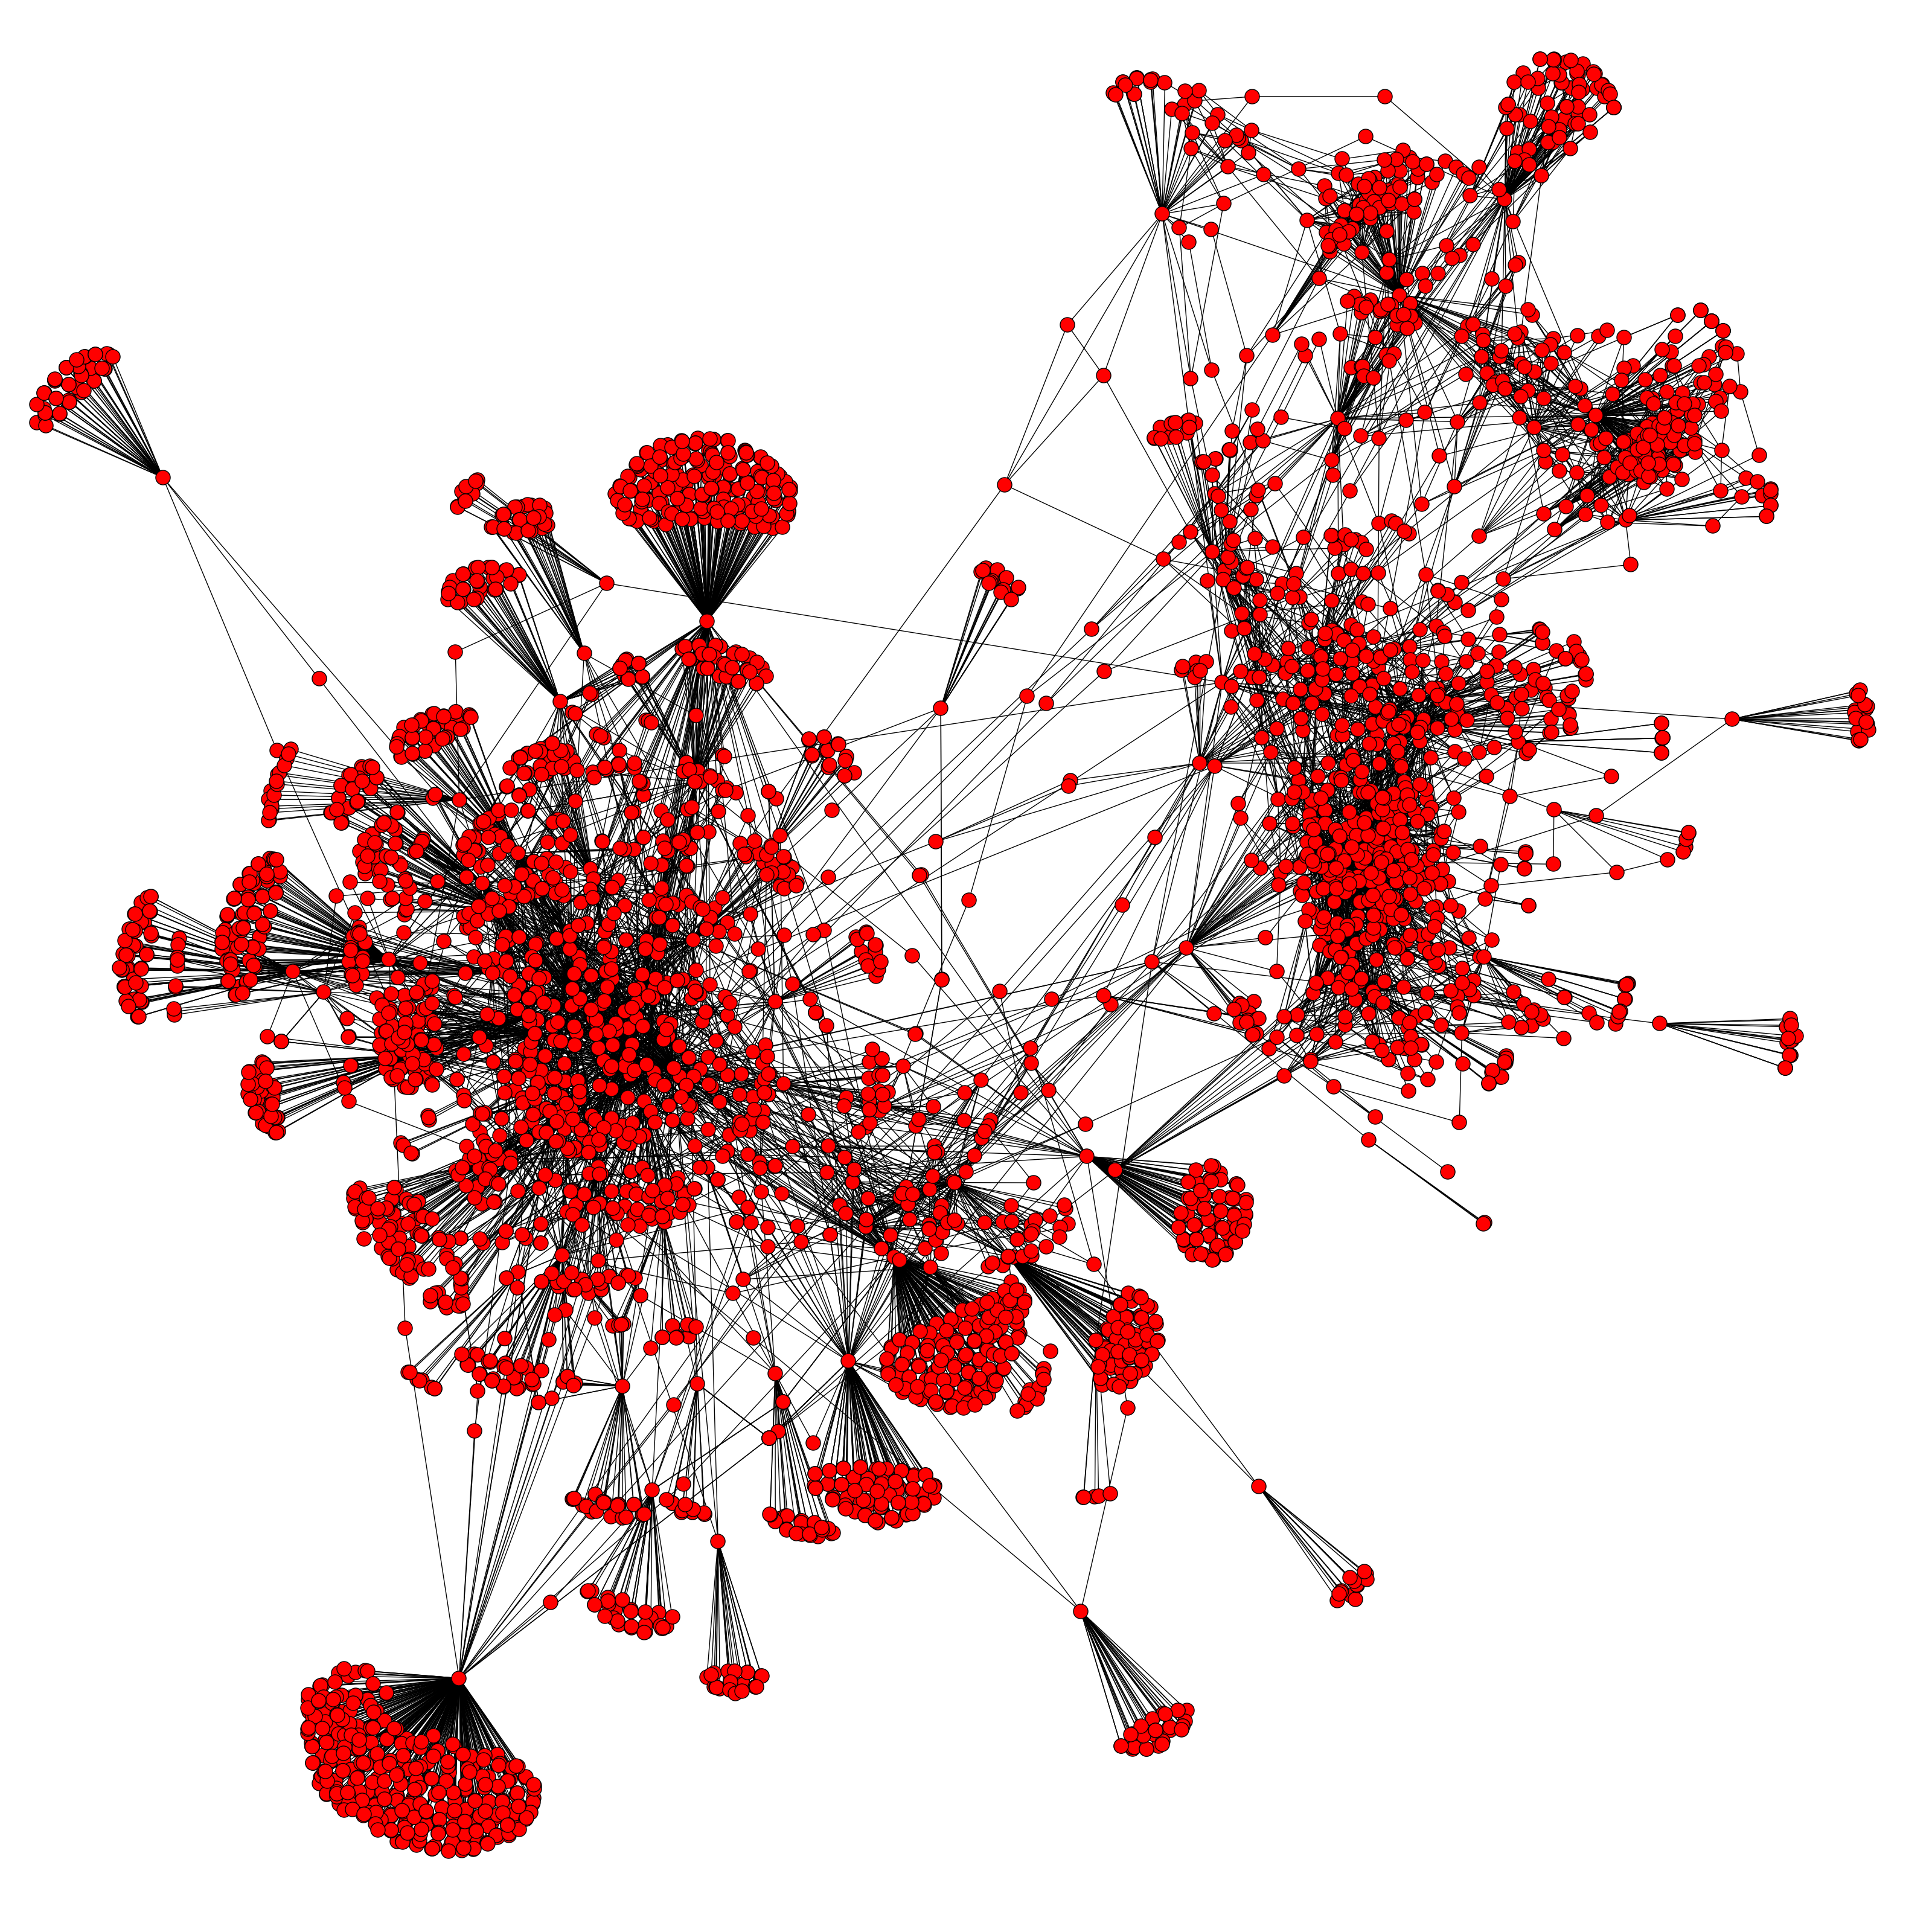
\includegraphics[width=0.7\textwidth]{pokec_4000}
  \caption{The subgraph constructed from the Pokec social network, using a breadth-first search limited to 4000 nodes. This network was used in place of a full real social network.}
  \label{fig:pokec_4000}
\end{figure}

Due to the size of the dataset, using the entire network was not feasible. To solve this, a subgraph was constructed. This was achieved by setting a limit on the number of nodes to include in the subgraph, in this case 4000, and then crawling the network in a breadth first manner, using the first node included in the dataset as a starting point. While the original data was directed, in this case it was treated as undirected - edges to or from nodes were considered to be undirected connections. The network created using the crawling process is shown in Figure \ref{fig:pokec_4000}. Of note is the fact that there are many nodes which are nearly disconnected from the rest of the graph, being only connected to single ``gateway" nodes. Interestingly, these ``gateway'' nodes tend to be connected to many such nearly-disconnected nodes. It is unclear whether this is an aspect of the original network or a result of the creation process. Since nodes added to the subgraph in the last step of the search would not have had all of their neighbours included, it is possible that these nearly-disconnected nodes have other connections which are not included in the subgraph. However these nodes must still have no mutual friends with their ``gateway'' node, which would be unusual. It is possible that the disconnected nodes represent ``abnormal" user accounts, such as those which do not represent real people. Alternatively, the it may be the ``gateway" nodes which are ``abnormal" - for example famous people who have many otherwise unconnected friends. Further work on the topic may be able to investigate this aspect in detail.

\begin{figure}
\begin{subfigure}[]{0.41\textwidth}
\captionsetup{justification=centering}
\begin{tikzpicture}
\begin{axis}[percentgraph,xmin=0,xmax=1,xlabel={$p_{further}$},legend pos=outer north east]
\addplot table [x=Not Closer Show Probability, y=average delivered (percent), col sep=comma] {results/pokec4000/not_closer_prob/2000messages.csv};
\addplot table [x=Not Closer Show Probability, y=average delivered (percent), col sep=comma] {results/pokec4000/not_closer_prob/4000messages.csv};
\addplot table [x=Not Closer Show Probability, y=average delivered (percent), col sep=comma] {results/pokec4000/not_closer_prob/6000messages.csv};
\addplot table [x=Not Closer Show Probability, y=average delivered (percent), col sep=comma] {results/pokec4000/not_closer_prob/8000messages.csv};
\end{axis}
\end{tikzpicture}
\caption{Algorithm 2 - Further Nodes With Probability}
\end{subfigure}
\quad1
\begin{subfigure}[]{0.41\textwidth}
\captionsetup{justification=centering}
\begin{tikzpicture}
\begin{axis}[percentgraph,xmin=0,xmax=1,xlabel={$f$},legend pos=outer north east,legend image post style={sharp plot},]
\addlegendimage{empty legend}
\addplot table [x=Distance Priority Fraction, y=average delivered (percent), col sep=comma] {results/pokec4000/distance_priority_fraction/2000messages.csv};
\addplot table [x=Distance Priority Fraction, y=average delivered (percent), col sep=comma] {results/pokec4000/distance_priority_fraction/4000messages.csv};
\addplot table [x=Distance Priority Fraction, y=average delivered (percent), col sep=comma] {results/pokec4000/distance_priority_fraction/6000messages.csv};
\addplot table [x=Distance Priority Fraction, y=average delivered (percent), col sep=comma] {results/pokec4000/distance_priority_fraction/8000messages.csv};
\legend{\hspace{-.6cm}\textbf{Messages},2000,4000,6000,8000}
\end{axis}
\end{tikzpicture}
\caption{Algorithm 5 - Fractional Distance Priority}
\end{subfigure}
\caption{Message delivery rates on the social network subgraph as the parameters for Algorithm 2 and Algorithm 5 are varied. For both $p_{further}$ and $f$, the optimal values were found to be 0.3.}
\label{fig:pokec_4000_params}
\end{figure}

As in previous cases, experiments were run to determine the best value of the parameters for Algorithm 2 (Further Nodes With Probability) and Algorithm 5 (Fractional Distance Priority), the results of which are shown in Figure \ref{fig:pokec_4000_params}. Simulations were run increased the values of $p_{further}$ for Algorithm 2 and $f$ for Algorithm 5 from 0 to in steps of 0.1. In this case, due to the size of the graph and long runtime resulting from this, experiments could only be repeated 5 times rather than the usual 20. These experiments were repeated and message counts of 2000 (half the number of nodes), 4000, 6000, and 8000 (double the number of nodes. It was found that the best values were $p_{further}=0.3$ and $f=0.3$. These values are different from what was found in previous cases - this is particularly interesting for $f$, which was found to be either optimal at 0.2 or make no difference in every other case considered. However the differences in delivery rates between $f=0.2$ and $f=0.2$ in this case were minimal, and may be effected by random fluctuation.

\begin{figure}
\centering
\begin{tikzpicture}
\begin{axis}[percentgraph,xmin=0,xmax=8000,xlabel={Message Count},width=0.75\textwidth,legend pos=north east]
\addplot table [x=Message count, y=average delivered (percent), col sep=comma] {results/pokec4000/FurtherProb_30.csv};
\addplot table [x=Message count, y=average delivered (percent), col sep=comma] {results/pokec4000/FractionalDistancePriority_30.csv};
\legend{Algorithm 2, Algorithm 5}
\end{axis}
\end{tikzpicture}
\caption{Delivery rates of Algorithm 2 and Algorithm 5 on the social network subgraph as message count is varied. Overall the performance on this graph was found to be lower than in similar experiments run using Kleinberg's graph model.}
\label{fig:pokec_4000_results}
\end{figure}

With the parameters set, experiments were run using Algorithm 2 and Algorithm 5 to measure their performance, the results of which are shown in Figure \ref{fig:pokec_4000_results}. These were conducted using message counts ranging from 500 to 8000, with intervals of 500. Again, it was only possible to repeat each experiment 5 times. As seen in other cases, Algorithm 5 outperformed Algorithm 2 significantly. However delivery rates for this graph were found to be significantly lower than those for Kleinberg's graph, even at low message counts. The delivery rates for Algorithm 2 ranged from 48.1\% to 9.0\%, and for Algorithm 5 from 58.8\% to 16.4\%.

As noted before, the new graph was found to contain many nearly-disconnected nodes connected only to single other ``gateway" nodes. If these nodes are a result of the process of creating the subgraph then this may contribute to the lower than expected delivery rates. However it is also possible that these cases do exist within the social network. In that case the results found would suggest that the Kleinberg model of social networks lacks certain aspects which have an effect on these algorithms.

\chapter{Conclusion} \label{chapter5}
We have defined our model of message sharing and selection, and described several display algorithms. Our results from conducting simulations of this message sharing process on Kleinberg's network model have shown that algorithms combining deterministic choice (to deliver messages quickly) with randomised aspects (to spread and keep messages alive) achieve the highest delivery rates. In particular Algorithm 5 (Fractional Distance Priority) which chooses a fraction of messages based on which is closest to the destination, and a the remainder at random, was found to perform best out of those tested. In most cases we found that setting the fraction of messages picked based on distance to 0.2 provides the best results, suggesting that only small amounts deterministic choices are required for optimal throughput - in fact even choosing a single message based on distance and the rest randomly performed well. This result is interesting, as it may mean that a small amount of distance based displaying could be mixed in with a normal (whatever the social network normally uses) display algorithm to help direct messages.

In addition to Kleinberg's model, we considered other graph types - chains, trees, and grids. In the case of chains, and to a lesser degree trees, we found that the low degree of the nodes severely limits the ability to spread messages, and as a result makes the choice of display algorithm almost irrelevant. We also ran simulations using a portion of a real social network. We found that performance on this network was lower than had been seen when using Kleinberg's model, however it was not clear if this was due to the fact that only part of the social network was used or differences between the model and real social networks.

\section{Further Work}
An obvious possibility for further work is the development of more display algorithms. For example, an algorithm could consider how many copies of a message currently exist in the graph, and use this to spread messages that have are almost lost more. In additional to developing display algorithms, other aspects have potential for more research.

While this study focused on experimental evaluation of algorithms, theoretical analysis may provide additional insights. In particular, analysis of the graph may be able to provide insights into the optimal achievable delivery rates, providing further opportunities to evaluate the success of display algorithms. It may also be possible to relate this model of message sharing to other similar models such as flow networks. This aspects were considered as part of this project, but time constraints did not allow any significant progress to be made.

Due to the number of parameters involved in the system, some were not considered in depth.
In particular, the graph parameters (such and size and number of long links added) may have some effect on the performance of algorithms or which algorithm parameters are optimal. The user model parameters (attention limit, probability of sharing messages) may also have similar effect. Future works could consider these aspects in more depth.

There were also some results found during this project which it was not possible to fully explain. For example, the exact reason that diffusion distance performs worse than graph distance was not clear, nor was the fact that message count affects delivery rates on tree graphs, but choice of algorithm largely does not. More detailed investigation of these cases may provide additional information on how aspects of the model interact.

Finally, it was found that the developed algorithms performed poorly on a portion of a real social network compared to Kleinberg's model, however the reason was not clear. It is possible that the model does not accurately replicate aspects of the social network which affect these algorithms, but it may also be that using only part of the network resulted in the subgraph having different properties. Analysis of how messages spread in this network and of any differences between this network and Kleinberg's model may be able to explain this result.

% use the following and \cite{} as above if you use BibTeX
% otherwise generate bibtem entries
\bibliographystyle{plain}
\bibliography{reportBib}


\end{document}
